\documentclass[10pt]{article} % For LaTeX2e
\usepackage[preprint]{tmlr}
% If accepted, instead use the following line for the camera-ready submission:
%\usepackage[accepted]{tmlr}
% To de-anonymize and remove mentions to TMLR (for example for posting to preprint servers), instead use the following:
%\usepackage[preprint]{tmlr}

% Optional math commands from https://github.com/goodfeli/dlbook_notation.
%%%%% NEW MATH DEFINITIONS %%%%%

\usepackage{amsmath,amsfonts,bm}

% Mark sections of captions for referring to divisions of figures
\newcommand{\figleft}{{\em (Left)}}
\newcommand{\figcenter}{{\em (Center)}}
\newcommand{\figright}{{\em (Right)}}
\newcommand{\figtop}{{\em (Top)}}
\newcommand{\figbottom}{{\em (Bottom)}}
\newcommand{\captiona}{{\em (a)}}
\newcommand{\captionb}{{\em (b)}}
\newcommand{\captionc}{{\em (c)}}
\newcommand{\captiond}{{\em (d)}}

% Highlight a newly defined term
\newcommand{\newterm}[1]{{\bf #1}}


% Figure reference, lower-case.
\def\figref#1{figure~\ref{#1}}
% Figure reference, capital. For start of sentence
\def\Figref#1{Figure~\ref{#1}}
\def\twofigref#1#2{figures \ref{#1} and \ref{#2}}
\def\quadfigref#1#2#3#4{figures \ref{#1}, \ref{#2}, \ref{#3} and \ref{#4}}
% Section reference, lower-case.
\def\secref#1{section~\ref{#1}}
% Section reference, capital.
\def\Secref#1{Section~\ref{#1}}
% Reference to two sections.
\def\twosecrefs#1#2{sections \ref{#1} and \ref{#2}}
% Reference to three sections.
\def\secrefs#1#2#3{sections \ref{#1}, \ref{#2} and \ref{#3}}
% Reference to an equation, lower-case.
\def\eqref#1{equation~\ref{#1}}
% Reference to an equation, upper case
\def\Eqref#1{Equation~\ref{#1}}
% A raw reference to an equation---avoid using if possible
\def\plaineqref#1{\ref{#1}}
% Reference to a chapter, lower-case.
\def\chapref#1{chapter~\ref{#1}}
% Reference to an equation, upper case.
\def\Chapref#1{Chapter~\ref{#1}}
% Reference to a range of chapters
\def\rangechapref#1#2{chapters\ref{#1}--\ref{#2}}
% Reference to an algorithm, lower-case.
\def\algref#1{algorithm~\ref{#1}}
% Reference to an algorithm, upper case.
\def\Algref#1{Algorithm~\ref{#1}}
\def\twoalgref#1#2{algorithms \ref{#1} and \ref{#2}}
\def\Twoalgref#1#2{Algorithms \ref{#1} and \ref{#2}}
% Reference to a part, lower case
\def\partref#1{part~\ref{#1}}
% Reference to a part, upper case
\def\Partref#1{Part~\ref{#1}}
\def\twopartref#1#2{parts \ref{#1} and \ref{#2}}

\def\ceil#1{\lceil #1 \rceil}
\def\floor#1{\lfloor #1 \rfloor}
\def\1{\bm{1}}
\newcommand{\train}{\mathcal{D}}
\newcommand{\valid}{\mathcal{D_{\mathrm{valid}}}}
\newcommand{\test}{\mathcal{D_{\mathrm{test}}}}

\def\eps{{\epsilon}}


% Random variables
\def\reta{{\textnormal{$\eta$}}}
\def\ra{{\textnormal{a}}}
\def\rb{{\textnormal{b}}}
\def\rc{{\textnormal{c}}}
\def\rd{{\textnormal{d}}}
\def\re{{\textnormal{e}}}
\def\rf{{\textnormal{f}}}
\def\rg{{\textnormal{g}}}
\def\rh{{\textnormal{h}}}
\def\ri{{\textnormal{i}}}
\def\rj{{\textnormal{j}}}
\def\rk{{\textnormal{k}}}
\def\rl{{\textnormal{l}}}
% rm is already a command, just don't name any random variables m
\def\rn{{\textnormal{n}}}
\def\ro{{\textnormal{o}}}
\def\rp{{\textnormal{p}}}
\def\rq{{\textnormal{q}}}
\def\rr{{\textnormal{r}}}
\def\rs{{\textnormal{s}}}
\def\rt{{\textnormal{t}}}
\def\ru{{\textnormal{u}}}
\def\rv{{\textnormal{v}}}
\def\rw{{\textnormal{w}}}
\def\rx{{\textnormal{x}}}
\def\ry{{\textnormal{y}}}
\def\rz{{\textnormal{z}}}

% Random vectors
\def\rvepsilon{{\mathbf{\epsilon}}}
\def\rvtheta{{\mathbf{\theta}}}
\def\rva{{\mathbf{a}}}
\def\rvb{{\mathbf{b}}}
\def\rvc{{\mathbf{c}}}
\def\rvd{{\mathbf{d}}}
\def\rve{{\mathbf{e}}}
\def\rvf{{\mathbf{f}}}
\def\rvg{{\mathbf{g}}}
\def\rvh{{\mathbf{h}}}
\def\rvu{{\mathbf{i}}}
\def\rvj{{\mathbf{j}}}
\def\rvk{{\mathbf{k}}}
\def\rvl{{\mathbf{l}}}
\def\rvm{{\mathbf{m}}}
\def\rvn{{\mathbf{n}}}
\def\rvo{{\mathbf{o}}}
\def\rvp{{\mathbf{p}}}
\def\rvq{{\mathbf{q}}}
\def\rvr{{\mathbf{r}}}
\def\rvs{{\mathbf{s}}}
\def\rvt{{\mathbf{t}}}
\def\rvu{{\mathbf{u}}}
\def\rvv{{\mathbf{v}}}
\def\rvw{{\mathbf{w}}}
\def\rvx{{\mathbf{x}}}
\def\rvy{{\mathbf{y}}}
\def\rvz{{\mathbf{z}}}

% Elements of random vectors
\def\erva{{\textnormal{a}}}
\def\ervb{{\textnormal{b}}}
\def\ervc{{\textnormal{c}}}
\def\ervd{{\textnormal{d}}}
\def\erve{{\textnormal{e}}}
\def\ervf{{\textnormal{f}}}
\def\ervg{{\textnormal{g}}}
\def\ervh{{\textnormal{h}}}
\def\ervi{{\textnormal{i}}}
\def\ervj{{\textnormal{j}}}
\def\ervk{{\textnormal{k}}}
\def\ervl{{\textnormal{l}}}
\def\ervm{{\textnormal{m}}}
\def\ervn{{\textnormal{n}}}
\def\ervo{{\textnormal{o}}}
\def\ervp{{\textnormal{p}}}
\def\ervq{{\textnormal{q}}}
\def\ervr{{\textnormal{r}}}
\def\ervs{{\textnormal{s}}}
\def\ervt{{\textnormal{t}}}
\def\ervu{{\textnormal{u}}}
\def\ervv{{\textnormal{v}}}
\def\ervw{{\textnormal{w}}}
\def\ervx{{\textnormal{x}}}
\def\ervy{{\textnormal{y}}}
\def\ervz{{\textnormal{z}}}

% Random matrices
\def\rmA{{\mathbf{A}}}
\def\rmB{{\mathbf{B}}}
\def\rmC{{\mathbf{C}}}
\def\rmD{{\mathbf{D}}}
\def\rmE{{\mathbf{E}}}
\def\rmF{{\mathbf{F}}}
\def\rmG{{\mathbf{G}}}
\def\rmH{{\mathbf{H}}}
\def\rmI{{\mathbf{I}}}
\def\rmJ{{\mathbf{J}}}
\def\rmK{{\mathbf{K}}}
\def\rmL{{\mathbf{L}}}
\def\rmM{{\mathbf{M}}}
\def\rmN{{\mathbf{N}}}
\def\rmO{{\mathbf{O}}}
\def\rmP{{\mathbf{P}}}
\def\rmQ{{\mathbf{Q}}}
\def\rmR{{\mathbf{R}}}
\def\rmS{{\mathbf{S}}}
\def\rmT{{\mathbf{T}}}
\def\rmU{{\mathbf{U}}}
\def\rmV{{\mathbf{V}}}
\def\rmW{{\mathbf{W}}}
\def\rmX{{\mathbf{X}}}
\def\rmY{{\mathbf{Y}}}
\def\rmZ{{\mathbf{Z}}}

% Elements of random matrices
\def\ermA{{\textnormal{A}}}
\def\ermB{{\textnormal{B}}}
\def\ermC{{\textnormal{C}}}
\def\ermD{{\textnormal{D}}}
\def\ermE{{\textnormal{E}}}
\def\ermF{{\textnormal{F}}}
\def\ermG{{\textnormal{G}}}
\def\ermH{{\textnormal{H}}}
\def\ermI{{\textnormal{I}}}
\def\ermJ{{\textnormal{J}}}
\def\ermK{{\textnormal{K}}}
\def\ermL{{\textnormal{L}}}
\def\ermM{{\textnormal{M}}}
\def\ermN{{\textnormal{N}}}
\def\ermO{{\textnormal{O}}}
\def\ermP{{\textnormal{P}}}
\def\ermQ{{\textnormal{Q}}}
\def\ermR{{\textnormal{R}}}
\def\ermS{{\textnormal{S}}}
\def\ermT{{\textnormal{T}}}
\def\ermU{{\textnormal{U}}}
\def\ermV{{\textnormal{V}}}
\def\ermW{{\textnormal{W}}}
\def\ermX{{\textnormal{X}}}
\def\ermY{{\textnormal{Y}}}
\def\ermZ{{\textnormal{Z}}}

% Vectors
\def\vzero{{\bm{0}}}
\def\vone{{\bm{1}}}
\def\vmu{{\bm{\mu}}}
\def\vtheta{{\bm{\theta}}}
\def\va{{\bm{a}}}
\def\vb{{\bm{b}}}
\def\vc{{\bm{c}}}
\def\vd{{\bm{d}}}
\def\ve{{\bm{e}}}
\def\vf{{\bm{f}}}
\def\vg{{\bm{g}}}
\def\vh{{\bm{h}}}
\def\vi{{\bm{i}}}
\def\vj{{\bm{j}}}
\def\vk{{\bm{k}}}
\def\vl{{\bm{l}}}
\def\vm{{\bm{m}}}
\def\vn{{\bm{n}}}
\def\vo{{\bm{o}}}
\def\vp{{\bm{p}}}
\def\vq{{\bm{q}}}
\def\vr{{\bm{r}}}
\def\vs{{\bm{s}}}
\def\vt{{\bm{t}}}
\def\vu{{\bm{u}}}
\def\vv{{\bm{v}}}
\def\vw{{\bm{w}}}
\def\vx{{\bm{x}}}
\def\vy{{\bm{y}}}
\def\vz{{\bm{z}}}

% Elements of vectors
\def\evalpha{{\alpha}}
\def\evbeta{{\beta}}
\def\evepsilon{{\epsilon}}
\def\evlambda{{\lambda}}
\def\evomega{{\omega}}
\def\evmu{{\mu}}
\def\evpsi{{\psi}}
\def\evsigma{{\sigma}}
\def\evtheta{{\theta}}
\def\eva{{a}}
\def\evb{{b}}
\def\evc{{c}}
\def\evd{{d}}
\def\eve{{e}}
\def\evf{{f}}
\def\evg{{g}}
\def\evh{{h}}
\def\evi{{i}}
\def\evj{{j}}
\def\evk{{k}}
\def\evl{{l}}
\def\evm{{m}}
\def\evn{{n}}
\def\evo{{o}}
\def\evp{{p}}
\def\evq{{q}}
\def\evr{{r}}
\def\evs{{s}}
\def\evt{{t}}
\def\evu{{u}}
\def\evv{{v}}
\def\evw{{w}}
\def\evx{{x}}
\def\evy{{y}}
\def\evz{{z}}

% Matrix
\def\mA{{\bm{A}}}
\def\mB{{\bm{B}}}
\def\mC{{\bm{C}}}
\def\mD{{\bm{D}}}
\def\mE{{\bm{E}}}
\def\mF{{\bm{F}}}
\def\mG{{\bm{G}}}
\def\mH{{\bm{H}}}
\def\mI{{\bm{I}}}
\def\mJ{{\bm{J}}}
\def\mK{{\bm{K}}}
\def\mL{{\bm{L}}}
\def\mM{{\bm{M}}}
\def\mN{{\bm{N}}}
\def\mO{{\bm{O}}}
\def\mP{{\bm{P}}}
\def\mQ{{\bm{Q}}}
\def\mR{{\bm{R}}}
\def\mS{{\bm{S}}}
\def\mT{{\bm{T}}}
\def\mU{{\bm{U}}}
\def\mV{{\bm{V}}}
\def\mW{{\bm{W}}}
\def\mX{{\bm{X}}}
\def\mY{{\bm{Y}}}
\def\mZ{{\bm{Z}}}
\def\mBeta{{\bm{\beta}}}
\def\mPhi{{\bm{\Phi}}}
\def\mLambda{{\bm{\Lambda}}}
\def\mSigma{{\bm{\Sigma}}}

% Tensor
\DeclareMathAlphabet{\mathsfit}{\encodingdefault}{\sfdefault}{m}{sl}
\SetMathAlphabet{\mathsfit}{bold}{\encodingdefault}{\sfdefault}{bx}{n}
\newcommand{\tens}[1]{\bm{\mathsfit{#1}}}
\def\tA{{\tens{A}}}
\def\tB{{\tens{B}}}
\def\tC{{\tens{C}}}
\def\tD{{\tens{D}}}
\def\tE{{\tens{E}}}
\def\tF{{\tens{F}}}
\def\tG{{\tens{G}}}
\def\tH{{\tens{H}}}
\def\tI{{\tens{I}}}
\def\tJ{{\tens{J}}}
\def\tK{{\tens{K}}}
\def\tL{{\tens{L}}}
\def\tM{{\tens{M}}}
\def\tN{{\tens{N}}}
\def\tO{{\tens{O}}}
\def\tP{{\tens{P}}}
\def\tQ{{\tens{Q}}}
\def\tR{{\tens{R}}}
\def\tS{{\tens{S}}}
\def\tT{{\tens{T}}}
\def\tU{{\tens{U}}}
\def\tV{{\tens{V}}}
\def\tW{{\tens{W}}}
\def\tX{{\tens{X}}}
\def\tY{{\tens{Y}}}
\def\tZ{{\tens{Z}}}


% Graph
\def\gA{{\mathcal{A}}}
\def\gB{{\mathcal{B}}}
\def\gC{{\mathcal{C}}}
\def\gD{{\mathcal{D}}}
\def\gE{{\mathcal{E}}}
\def\gF{{\mathcal{F}}}
\def\gG{{\mathcal{G}}}
\def\gH{{\mathcal{H}}}
\def\gI{{\mathcal{I}}}
\def\gJ{{\mathcal{J}}}
\def\gK{{\mathcal{K}}}
\def\gL{{\mathcal{L}}}
\def\gM{{\mathcal{M}}}
\def\gN{{\mathcal{N}}}
\def\gO{{\mathcal{O}}}
\def\gP{{\mathcal{P}}}
\def\gQ{{\mathcal{Q}}}
\def\gR{{\mathcal{R}}}
\def\gS{{\mathcal{S}}}
\def\gT{{\mathcal{T}}}
\def\gU{{\mathcal{U}}}
\def\gV{{\mathcal{V}}}
\def\gW{{\mathcal{W}}}
\def\gX{{\mathcal{X}}}
\def\gY{{\mathcal{Y}}}
\def\gZ{{\mathcal{Z}}}

% Sets
\def\sA{{\mathbb{A}}}
\def\sB{{\mathbb{B}}}
\def\sC{{\mathbb{C}}}
\def\sD{{\mathbb{D}}}
% Don't use a set called E, because this would be the same as our symbol
% for expectation.
\def\sF{{\mathbb{F}}}
\def\sG{{\mathbb{G}}}
\def\sH{{\mathbb{H}}}
\def\sI{{\mathbb{I}}}
\def\sJ{{\mathbb{J}}}
\def\sK{{\mathbb{K}}}
\def\sL{{\mathbb{L}}}
\def\sM{{\mathbb{M}}}
\def\sN{{\mathbb{N}}}
\def\sO{{\mathbb{O}}}
\def\sP{{\mathbb{P}}}
\def\sQ{{\mathbb{Q}}}
\def\sR{{\mathbb{R}}}
\def\sS{{\mathbb{S}}}
\def\sT{{\mathbb{T}}}
\def\sU{{\mathbb{U}}}
\def\sV{{\mathbb{V}}}
\def\sW{{\mathbb{W}}}
\def\sX{{\mathbb{X}}}
\def\sY{{\mathbb{Y}}}
\def\sZ{{\mathbb{Z}}}

% Entries of a matrix
\def\emLambda{{\Lambda}}
\def\emA{{A}}
\def\emB{{B}}
\def\emC{{C}}
\def\emD{{D}}
\def\emE{{E}}
\def\emF{{F}}
\def\emG{{G}}
\def\emH{{H}}
\def\emI{{I}}
\def\emJ{{J}}
\def\emK{{K}}
\def\emL{{L}}
\def\emM{{M}}
\def\emN{{N}}
\def\emO{{O}}
\def\emP{{P}}
\def\emQ{{Q}}
\def\emR{{R}}
\def\emS{{S}}
\def\emT{{T}}
\def\emU{{U}}
\def\emV{{V}}
\def\emW{{W}}
\def\emX{{X}}
\def\emY{{Y}}
\def\emZ{{Z}}
\def\emSigma{{\Sigma}}

% entries of a tensor
% Same font as tensor, without \bm wrapper
\newcommand{\etens}[1]{\mathsfit{#1}}
\def\etLambda{{\etens{\Lambda}}}
\def\etA{{\etens{A}}}
\def\etB{{\etens{B}}}
\def\etC{{\etens{C}}}
\def\etD{{\etens{D}}}
\def\etE{{\etens{E}}}
\def\etF{{\etens{F}}}
\def\etG{{\etens{G}}}
\def\etH{{\etens{H}}}
\def\etI{{\etens{I}}}
\def\etJ{{\etens{J}}}
\def\etK{{\etens{K}}}
\def\etL{{\etens{L}}}
\def\etM{{\etens{M}}}
\def\etN{{\etens{N}}}
\def\etO{{\etens{O}}}
\def\etP{{\etens{P}}}
\def\etQ{{\etens{Q}}}
\def\etR{{\etens{R}}}
\def\etS{{\etens{S}}}
\def\etT{{\etens{T}}}
\def\etU{{\etens{U}}}
\def\etV{{\etens{V}}}
\def\etW{{\etens{W}}}
\def\etX{{\etens{X}}}
\def\etY{{\etens{Y}}}
\def\etZ{{\etens{Z}}}

% The true underlying data generating distribution
\newcommand{\pdata}{p_{\rm{data}}}
% The empirical distribution defined by the training set
\newcommand{\ptrain}{\hat{p}_{\rm{data}}}
\newcommand{\Ptrain}{\hat{P}_{\rm{data}}}
% The model distribution
\newcommand{\pmodel}{p_{\rm{model}}}
\newcommand{\Pmodel}{P_{\rm{model}}}
\newcommand{\ptildemodel}{\tilde{p}_{\rm{model}}}
% Stochastic autoencoder distributions
\newcommand{\pencode}{p_{\rm{encoder}}}
\newcommand{\pdecode}{p_{\rm{decoder}}}
\newcommand{\precons}{p_{\rm{reconstruct}}}

\newcommand{\laplace}{\mathrm{Laplace}} % Laplace distribution

\newcommand{\E}{\mathbb{E}}
\newcommand{\Ls}{\mathcal{L}}
\newcommand{\R}{\mathbb{R}}
\newcommand{\emp}{\tilde{p}}
\newcommand{\lr}{\alpha}
\newcommand{\reg}{\lambda}
\newcommand{\rect}{\mathrm{rectifier}}
\newcommand{\softmax}{\mathrm{softmax}}
\newcommand{\sigmoid}{\sigma}
\newcommand{\softplus}{\zeta}
\newcommand{\KL}{D_{\mathrm{KL}}}
\newcommand{\Var}{\mathrm{Var}}
\newcommand{\standarderror}{\mathrm{SE}}
\newcommand{\Cov}{\mathrm{Cov}}
% Wolfram Mathworld says $L^2$ is for function spaces and $\ell^2$ is for vectors
% But then they seem to use $L^2$ for vectors throughout the site, and so does
% wikipedia.
\newcommand{\normlzero}{L^0}
\newcommand{\normlone}{L^1}
\newcommand{\normltwo}{L^2}
\newcommand{\normlp}{L^p}
\newcommand{\normmax}{L^\infty}

\newcommand{\parents}{Pa} % See usage in notation.tex. Chosen to match Daphne's book.

\DeclareMathOperator*{\argmax}{arg\,max}
\DeclareMathOperator*{\argmin}{arg\,min}

\DeclareMathOperator{\sign}{sign}
\DeclareMathOperator{\Tr}{Tr}
\let\ab\allowbreak

% Restore standard parenthesized equation references overridden by math_commands.tex
\renewcommand{\eqref}[1]{(\ref{#1})}

\usepackage{amsmath,amssymb,amsfonts,amsthm}
\usepackage{booktabs}
\usepackage{multirow}
\usepackage{tabularx}
\usepackage{array}
\usepackage{graphicx}
\usepackage{microtype}
\usepackage{algorithm}
\usepackage{algpseudocode}
\usepackage{enumitem}
\usepackage{hyperref}
\usepackage{url}

\graphicspath{{figures/}}

% Independent theorem-like counters for clarity
\newtheorem{theorem}{Theorem}
\newtheorem{lemma}{Lemma}
\newtheorem{definition}{Definition}
\newtheorem{proposition}{Proposition}
\newtheorem{remark}{Remark}

\newcommand{\lean}{\textsc{Project LEAN}}
\newcommand{\kac}{\textsc{KAC}}
\newcommand{\gqakac}{\textsc{GQA-KAC}}
\newcommand{\pqv}{\textsc{Priced-Quanta v2}}
\newcommand{\glimmer}{\textsc{Muse-Glimmer-30B}}
\newcommand{\bpp}{\mathrm{bpp}}

\title{Priced-Quanta: Decoupling Algorithmic Routing from Associative Memory for Sub-4-Bit and 8 GiB Edge Language Model Serving}

% Authors must not appear in the submitted version. They should be hidden
% as long as the tmlr package is used without the [accepted] or [preprint] options.
% Non-anonymous submissions will be rejected without review.
\author{\name Mehardeep Singh \email github.com/Mehardeep-Singh-GG \\
      \addr Independent Researcher
      \AND
      \name Gurarpit Singh \email github.com/gurarpitzz \\
      \addr Independent Researcher}

\newcommand{\fix}{\marginpar{FIX}}
\newcommand{\new}{\marginpar{NEW}}

\def\month{MM}
\def\year{YYYY}
\def\openreview{\url{https://openreview.net/forum?id=XXXX}}

\begin{document}

\maketitle

\begin{abstract}
Uniform post-training quantization assigns identical bit-widths to attention routing projections and feed-forward multilayer perceptron (MLP) blocks, despite mechanistic evidence that MLPs primarily store static associative facts while attention executes context routing. We investigate this asymmetry theoretically and empirically across pretrained transformers spanning $70\text{M}$ to $29.78\text{B}$ parameters. Using a corrected Wedin $\sin\Theta$ subspace bound, a Cauchy--Schwarz argmax routing margin condition, and a first-order linearized MLP noise analysis, we characterize how rank-order attention routing tolerates perturbation differently from dense associative recall, and formalize mixed-precision allocation with external retrieval as a Multiple-Choice Knapsack Problem (\kac{}). Across checkpoints without tokenizer-floor artifacts (\texttt{Pythia-70M/160M}, \texttt{GPT-2}, near-chance \texttt{Pythia-410M}), progressive quantization degrades factual cloze faster than procedural lookup ($1.20\times$--$5.30\times$ transformer-bit half-life ratios), while our forensic audit flags a BPE first-token artifact on digit-splitting tokenizers (\texttt{SmolLM2}, \texttt{Qwen2.5}). At exact 4b/3b backbone bit parity ($\Delta=0.000\%$) paired with an idealized $17.81\,\text{KiB}$ BM25 store over the evaluation facts, \kac{} improves retrieval cloze on \texttt{Pythia-160M} ($+5.5\,\text{pp}$, $-1.50$ nats) and \texttt{SmolLM2-360M} ($+8.0\,\text{pp}$ raw, $+1.0\,\text{pp}$ retrieval). On \texttt{Qwen2.5-3B-Instruct}, MSE group clipping rescues 3-bit MLP collapse ($12.0\% \to 94.0\%$ across five seeds vs.\ $89.8\%$ for an unclipped prefix baseline; two-sided permutation $p=0.0625$), explicitly trading closed-book recall ($62.4\% \to 20.2\%$) and loss ($6.72 \to 9.45$ nats) for retrieval accuracy. On a physical $8.00\,\text{GiB}$ RTX 4060 GPU where FP16 \texttt{Qwen2.5-7B-Instruct} ($14.19\,\text{GiB}$) OOMs, 4b/2b AWQ-\gqakac{} fits in $3.84\,\text{GiB}$ weights ($4.34\,\text{GiB}$ allocated VRAM) and reaches $88.0\%$ retrieval cloze using 48 disjoint WikiText-2 sequences ($\alpha=0.4$ winning in $88.1\%$ of projections). Scaling to \glimmer{} ($29.78\text{B}$, $55.46\,\text{GiB}$ BF16), greedy Lagrangian allocation yields a $6.08\,\text{GiB}$ ($1.754\,\bpp$) blueprint, damped Block-Cholesky Hessian compensation cuts in-sample calibration output error by $47.0\%$ across eight real sliced projections, and a deferred-reduction Split-K fused Triton daemon executes all 52 real text layers beneath an $8.00\,\text{GiB}$ GPU cap ($7.29\,\text{GiB}$ PyTorch / $7.92\,\text{GiB}$ \texttt{nvidia-smi} + $3.26\,\text{GiB}$ host CPU offload, $9.0\,\text{tok/s}$). We disclose all preregistered misses, calibration overlaps, and protocol limitations transparently.
\end{abstract}

\section{Introduction}
\label{sec:intro}

Running multi-billion-parameter autoregressive transformers \citep{vaswani2017attention} on consumer $8.00\,\text{GiB}$ GPUs is fundamentally bounded by memory capacity: static 16-bit weights alone require $14.19\,\text{GiB}$ at $7.6\text{B}$ and $55.46\,\text{GiB}$ at $29.78\text{B}$. Existing workarounds expose a sharp trade-off: out-of-core layer offloading \citep{sheng2023flexgen} incurs PCIe stalls, whereas uniform post-training quantization (PTQ)---GPTQ \citep{frantar2023gptq}, AWQ \citep{lin2024awq}, SmoothQuant \citep{xiao2023smoothquant}, HQQ \citep{badri2023hqq}, QuIP/QuIP\# \citep{chee2023quip,tseng2024quipsharp}, and AQLM \citep{egiazarian2024aqlm}---assigns identical precision across attention and feed-forward MLP blocks.

Mechanistic interpretability motivates asymmetric allocation. Prior work shows that MLPs act substantially as key-value associative memories \citep{geva2021transformer,meng2022locating} storing static facts in superposition \citep{elhage2022superposition}---though localization is non-strict \citep{hase2023localization}---while attention heads execute induction and context copying \citep{olsson2022incontext,ainslie2023gqa}. Independently, compression degrades long-tail factual recall disproportionately \citep{kandpal2023large,jaiswal2024compressing}. Because SwiGLU MLPs occupy $75\%$--$86\%$ of non-embedding transformer weights whereas Grouped-Query Attention (GQA) key-value projections occupy under $1\%$ while serving $8\times$--$16\times$ as many query heads, uniform bit assignment misallocates scarce edge bits.

We introduce \lean{} (\emph{Low-bit Externalized Associative Network}) and the \emph{Priced-Quanta} formulation: we externalize static factual lookup to a deterministic BM25 index \citep{robertson2009bm25}, compress MLPs aggressively ($1.58$--$3$ bits), and reallocate bits to protect attention routing under a Multiple-Choice Knapsack budget. Strictly scoped to verified artifacts, our contributions span: (1) formal perturbation asymmetry and greedy MCKP guarantees backed by synthetic scaling and an audited 18-entry preregistration ledger (Section~\ref{sec:theory}, Appendices~\ref{app:proofs}--\ref{app:controlled}); (2) cross-family survival asymmetry ($1.20\times$--$5.30\times$), a forensic BPE tokenizer audit, byte-parity 4b/3b compression up to $3\text{B}$, and leak-free WikiText-2 AWQ 4b/2b serving of \texttt{Qwen2.5-7B-Instruct} on a physical $8.00\,\text{GiB}$ RTX 4060 GPU (Section~\ref{sec:real_llms}); and (3) 52-layer spectral profiling, Block-Cholesky Hessian compensation ($-47.0\%$ macro calibration output error), and live Split-K fused Triton GPU serving of \glimmer{} under an $8.00\,\text{GiB}$ GPU cap (Section~\ref{sec:30b_scale}).

\section{Theoretical Framework: Functional Asymmetry and Priced-Quanta Allocation}
\label{sec:theory}

\subsection{Definitions and Layer-Wise Surrogate Model}
\label{sec:theory_defs}

Consider an $L$-layer autoregressive transformer with hidden width $d$, head dimension $d_k$, $H_q$ query heads, $H_{kv}$ key-value heads (GQA mapping $g(h) \in \{1,\dots,H_{kv}\}$ for $h \in \{1,\dots,H_q\}$), and SwiGLU width $d_{\text{mlp}}$. Throughout, inputs are column vectors $\vx \in \R^{d_{\text{in}}}$, weights are $\mW \in \R^{d_{\text{out}} \times d_{\text{in}}}$, and quantization residuals follow $\mE \equiv \mW - \widehat{\mW}$ (so $\widehat{\mW} = \mW - \mE$).

\begin{definition}[Group-Wise Weight Quantization]
\label{def:quant}
For $\mW \in \R^{d_{\text{out}} \times d_{\text{in}}}$, group size $g_{\text{sz}}$, and bit-width $b \in \{1, \log_2 3, 2, 3, 4, 6, 8, 16\}$, group-wise quantization partitions each row into $G_r = \lceil d_{\text{in}} / g_{\text{sz}} \rceil$ contiguous blocks with per-group scale $s_k$ (and optional offset $z_k$), yielding $\widehat{\mW} = \mW - \mE$. Under high-rate Bennett white-noise assumptions (a first-order analytical baseline that extrapolates only approximately to heavy-tailed $b \le 2$ weights), entrywise noise variance scales as $\sigma_E^2(b) \propto 2^{-2b}$.
\end{definition}

Following \citet{frantar2023gptq}, each linear layer $i$ is optimized under the layer-wise output MSE surrogate over $N_{\text{cal}}$ calibration tokens stacked as rows of $\mX_i \in \R^{N_{\text{cal}} \times d_{\text{in}}}$:
\begin{equation}
    \mathcal{E}_{\text{out}}(\widehat{\mW}_i)
    = \frac{1}{N_{\text{cal}}} \big\| (\mW_i - \widehat{\mW}_i)\mX_i^\top \big\|_F^2
    = \frac{1}{2}\,\mathrm{Tr}\!\left(\mH_i\,\mE_i^\top \mE_i\right),
    \qquad
    \mH_i \equiv \frac{2}{N_{\text{cal}}}\mX_i^\top \mX_i \succeq \mathbf{0},
    \label{eq:hessian_loss}
\end{equation}
where $\mH_i \in \R^{d_{\text{in}} \times d_{\text{in}}}$ is the uncentered input Gram matrix. Avoiding isotropic cross-layer curvature assumptions ($\nabla^2_{\vy_i}\mathcal{L} \propto \mI$), cross-layer functional importance is encoded via explicit leverage weights $\omega_i \ge 0$ in Section~\ref{sec:theory_knapsack}.

\begin{definition}[Dual-Operator Sub-Block Decomposition]
\label{def:dual}
Within decoder layer $\ell$ (evaluated on exact single-layer inputs $\vx_1,\dots,\vx_t \in \R^d$ without positional rotation for analytical clarity), we contrast:
\begin{enumerate}[leftmargin=*,nosep]
    \item \textbf{Bilinear attention routing:} Head $h$ with per-head projections $\mW_q^{(h)}, \mW_k^{(g(h))}, \mW_v^{(g(h))} \in \R^{d_k \times d}$ and output slice $\mW_o^{(h)} \in \R^{d \times d_k}$ defines $\mM^{(h)} = (\mW_q^{(h)})^\top \mW_k^{(g(h))} \in \R^{d \times d}$, logits $S_{t,j}^{(h)} = d_k^{-1/2} \vx_t^\top \mM^{(h)} \vx_j$, attention weights $A_{t,:}^{(h)} = \mathrm{softmax}(S_{t,:}^{(h)})$, and output $\vy_{\text{attn}}^{(h)} = \mW_o^{(h)} \sum_{j \le t} A_{t,j}^{(h)} \mW_v^{(g(h))} \vx_j$. (With Rotary Position Embeddings, \citealp{su2024roformer}, $\mM_{t-j}^{(h)} = (\mW_q^{(h)})^\top \mR_{t-j} \mW_k^{(g(h))}$ with $\|\mR_{t-j}\|_2 = 1$.)
    \item \textbf{MLP key-value associative memory:} A gated SwiGLU block computes $\vy_{\text{mlp}}(\vx) = \sum_{m=1}^{d_{\text{mlp}}} \vv_m\,\phi(\vk_m^\top \vx, \vu_m^\top \vx)$ with $\phi(a, b) = \mathrm{SiLU}(a)\cdot b$ and $\vv_m = (\mW_{\text{down}})_{:,m}$ \citep{geva2021transformer}. For analytical tractability in Theorem~\ref{thm:asymmetry}, we analyze the single-activation readout $\vy_{\text{mlp}}(\vx) = \sum_{m=1}^{d_{\text{mlp}}} \vv_m\,\psi(\vk_m^\top \vx)$ with $L_\psi$-Lipschitz activation $\psi$.
\end{enumerate}
\end{definition}

\begin{definition}[Operational Quantization Survival Half-Life]
\label{def:halflife}
For a task family $\mathcal{T}$ with FP16 accuracy $A_0 > A_{\text{chance}}$, let retention along a discrete ladder $\{b_k\}$ be raw $R_{\mathcal{T}}^{\text{raw}}(b) = A(b)/A_0$ or chance-corrected $R_{\mathcal{T}}^{\text{exc}}(b) = (A(b) - A_{\text{chance}})/(A_0 - A_{\text{chance}})$. The half-life $h_{1/2}(\mathcal{T})$ (or bit budget $B_{1/2}(\mathcal{T})$) is the piecewise-linear threshold where $R_{\mathcal{T}}$ first reaches $0.50$. If a curve never crosses $0.50$ down to $b_{\min}$, $B_{1/2}$ is uncrossed and bounded above by $b_{\min}$ (any extrapolated ratios are flagged explicitly in Section~\ref{sec:cross_family} and Appendix~\ref{app:controlled}).
\end{definition}

\subsection{Perturbation Asymmetry Between Attention Routing and Associative Recall}
\label{sec:theory_thm}

\begin{theorem}[Single-Layer Attention Routing Stability vs.\ Linearized MLP Noise Sensitivity]
\label{thm:asymmetry}
Consider a single NoPE transformer layer evaluated on exact context vectors $\{\vx_j\}_{j=1}^{t}$ with radius $R_x = \max_{1 \le j \le t} \|\vx_j\|_2$.
\begin{enumerate}[leftmargin=*,nosep]
    \item \textbf{Attention subspace stability and argmax routing invariance:} Let $\mM = \mW_q^\top \mW_k \in \R^{d \times d}$ have singular values $\sigma_1(\mM) > \sigma_2(\mM) \ge \dots \ge 0$ with spectral gap $\Delta\sigma = \sigma_1(\mM) - \sigma_2(\mM) > 0$, and let $\mE_M \equiv \widehat{\mM} - \mM = -\mE_q^\top \mW_k - \mW_q^\top \mE_k + \mE_q^\top \mE_k$.
    \begin{enumerate}[label=(\alph*),leftmargin=*,nosep]
        \item Whenever $\|\mE_M\|_2 < \Delta\sigma$, Wedin's $\sin\Theta$ theorem \citep{wedin1972perturbation} guarantees leading singular subspace stability:
        \begin{equation}
            \max\!\big\{\sin\Theta(\vu_1, \widehat{\vu}_1),\; \sin\Theta(\vv_1, \widehat{\vv}_1)\big\} \le \frac{\|\mE_M\|_2}{\Delta\sigma - \|\mE_M\|_2}.
            \label{eq:wedin_bound}
        \end{equation}
        \item Independently of \eqref{eq:wedin_bound}, for query $\vx_t$ with unique unperturbed target $j^* = \arg\max_j S_{t,j}$ and margin $\gamma_{\min} = \min_{j \ne j^*}(S_{t,j^*} - S_{t,j}) > 0$, the discrete argmax routing decision is strictly invariant ($\arg\max_j \widehat{A}_{t,j} = j^*$) whenever
        \begin{equation}
            \|\mE_M\|_2 < \frac{\gamma_{\min}\sqrt{d_k}}{2 R_x^2}.
            \label{eq:attn_margin}
        \end{equation}
    \end{enumerate}
    \item \textbf{First-order linearized MLP associative noise:} Consider $\vy(\vx) = \sum_{m=1}^{d_{\text{mlp}}} \vv_m \psi(\vk_m^\top \vx)$ perturbed by independent zero-mean per-column noise with covariances $\E[\ve_{v,m}\ve_{v,m'}^\top] = \delta_{m,m'}\sigma_E^2 \mI_d$ and $\E[\ve_{k,m}\ve_{k,m'}^\top] = \delta_{m,m'}\sigma_E^2 \mI_{d_{\text{in}}}$, independent of $\vx$. Evaluating the first-order linearized readout $\widehat{\vy}_{\text{lin}}(\vx) = \sum_{m=1}^{d_{\text{mlp}}} (\vv_m - \ve_{v,m})(\psi(\vk_m^\top \vx) - \psi'(\vk_m^\top \vx)(\ve_{k,m}^\top \vx))$ (exact for piecewise-linear $\psi$ within a linear region) around target association $m^*$, $\bm{\eta}_{\text{lin}} = \widehat{\vy}_{\text{lin}}(\vx) - \vy(\vx)$ satisfies
    \begin{equation}
        \E[\|\bm{\eta}_{\text{lin}}\|_2^2]
        = \sigma_E^2 \sum_{m=1}^{d_{\text{mlp}}} \|\vv_m\|_2^2\,\E\!\big[\psi'(\vk_m^\top \vx)^2 \|\vx\|_2^2\big]
        + d\,\sigma_E^2 \sum_{m=1}^{d_{\text{mlp}}} \E\!\big[\psi(\vk_m^\top \vx)^2\big]
        + \mathcal{O}(\sigma_E^4),
        \label{eq:mlp_noise}
    \end{equation}
    yielding the first-order total-norm associative SINR
    \begin{equation}
        \mathrm{SINR}_{\text{fact}}(b)
        = \frac{\|\vv_{m^*}\|_2^2\,\E[\psi(\vk_{m^*}^\top \vx)^2]}{\mathcal{I}_{\text{crosstalk}} + \sigma_E^2(b)\!\left(\sum_{m=1}^{d_{\text{mlp}}} \|\vv_m\|_2^2\,\E[\psi'(\vk_m^\top \vx)^2 \|\vx\|_2^2] + d \sum_{m=1}^{d_{\text{mlp}}}\E[\psi(\vk_m^\top \vx)^2]\right) + \mathcal{O}(\sigma_E^4)},
        \label{eq:mlp_sinr}
    \end{equation}
    where $\mathcal{I}_{\text{crosstalk}} = \E[\|\sum_{j \ne m^*} \vv_j \psi(\vk_j^\top \vx)\|_2^2]$. Projecting onto unit decoding vector $\vu_{m^*} = \vv_{m^*}/\|\vv_{m^*}\|_2$ replaces $d$ by $1$ in the value-noise term, $\|\vv_m\|_2^2$ by $(\vu_{m^*}^\top \vv_m)^2$ in the key-noise term, and $\mathcal{I}_{\text{crosstalk}}$ by $\E[(\vu_{m^*}^\top \bm{\xi})^2]$, while retaining the full sum over all $d_{\text{mlp}}$ superimposed neurons.
\end{enumerate}
\end{theorem}

The full proof and Softmax Jacobian Lemma (Lemma~\ref{lem:softmax}: $\|\mJ\|_2 \le 2\epsilon$ for $\max_j a_j = 1-\epsilon$) appear in Appendix~\ref{app:proofs}.

\begin{remark}[Mechanistic Interpretation and Architectural Caveats]
\label{rem:mechanistic}
Theorem~\ref{thm:asymmetry} highlights two structural contrasts without claiming a universal closed-form bit threshold. First, attention routing requires only preserving a finite argmax margin \eqref{eq:attn_margin} over in-context tokens, whereas MLP associative recall accumulates noise across all $d_{\text{mlp}}$ superimposed neurons against crosstalk $\mathcal{I}_{\text{crosstalk}}$ \citep{elhage2022superposition}. Second, under GQA ($H_{kv} \ll H_q$), quantizing $\mW_k$ corrupts $\mE_M$ across all $H_q / H_{kv}$ shared query heads while quantizing $\mW_v$ perturbs $\vy_{\text{attn}}^{(h)}$ across those same heads. Conversely, (i) SwiGLU ($\mathrm{SiLU}(a)\cdot b$) has unbounded gradients as $|b| \to \infty$ and $b \in \{1.585, 2\}$ violates small-$\sigma_E$ linearization, and (ii) residual streams accumulate input errors $\Delta\vx_t$ across depth---motivating the empirical calibration and Hessian compensation in Sections~\ref{sec:real_llms} and~\ref{sec:30b_scale}.
\end{remark}

\subsection{Multiple-Choice Knapsack Bit Allocation and Systems Primitives}
\label{sec:theory_knapsack}

Given byte budget $B_{\text{target}}$ and external index size $S_{\text{index}}$, we assign each projection $i \in \{1,\dots,M\}$ a precision $b \in \mathcal{P}_i$ with byte cost $S_i(b)$ and utility $v_i(b) = -\omega_i D_i(b) \le 0$ ($\omega_i \ge 0$, $D_i(b) \ge 0$):
\begin{equation}
    \max_{\{x_{i,b} \in \{0,1\}\}} \sum_{i=1}^{M} \sum_{b \in \mathcal{P}_i} x_{i,b}\, v_i(b)
    \quad \text{subject to} \quad
    \sum_{b \in \mathcal{P}_i} x_{i,b} = 1\;\forall i, \quad
    \sum_{i=1}^{M} \sum_{b \in \mathcal{P}_i} x_{i,b}\, S_i(b) + S_{\text{index}} \le B_{\text{target}}.
    \label{eq:mckp}
\end{equation}

\begin{proposition}[LP-Relaxation Optimality Bound of Efficiency-Sorted Greedy MCKP]
\label{prop:knapsack}
Assume \eqref{eq:mckp} is feasible ($\sum_{i=1}^{M} \min_{b \in \mathcal{P}_i} S_i(b) + S_{\text{index}} \le B_{\text{target}}$) with $\omega_i \ge 0, D_i(b) \ge 0$. After discarding simple- and LP-dominated options within each $\mathcal{P}_i$ so only strictly increasing LP-undominated upper-concave-hull choices remain, initializing at minimum cost and greedily applying upgrades $b \to b'$ in descending marginal efficiency $e_i(b \to b') = (v_i(b') - v_i(b))/(S_i(b') - S_i(b))$ until the next upgrade exceeds $B_{\text{target}}$ yields objective $V_{\mathrm{Greedy}}$ within
\begin{equation}
    V_{\mathrm{DP}}^* - V_{\mathrm{Greedy}} \le \max_{i \in \{1,\dots,M\}} \max_{b_1, b_2 \in \mathcal{P}_i} \big(v_i(b_2) - v_i(b_1)\big)
    \label{eq:knapsack_gap}
\end{equation}
of the exact integer optimum $V_{\mathrm{DP}}^*$ (proof in Appendix~\ref{app:knapsack_proof}).
\end{proposition}

Our practical pipeline pairs this greedy Lagrangian allocator (used directly in \texttt{M15} rather than pseudo-polynomial DP over $6.5\times 10^9$ byte states) with four primitives (detailed in Appendix~\ref{app:algorithms}): (1) \textbf{AWQ-KAC} channel rescaling $\mW' = \mW\,\mathrm{diag}(\vs)$, $\vs = (\vs_x / \bar{s}_x)^\alpha$ ($\alpha \in \{0.4, 0.5, 0.6, 0.75\}$; \citealp{lin2024awq}) plus vectorized group MSE clipping; (2) \textbf{Damped Block-Cholesky Hessian compensation with sparse outliers} (Algorithm~\ref{alg:cholesky}), extracting top $\rho \in \{0.35\%, 0.50\%\}$ salient columns $\mathcal{O}$ by $\|\mW_{:,j}\|_2\|\mX_{:,j}\|_2$, factoring $\mH_{\mathcal{O}^c,\mathcal{O}^c}^{-1} = \mU^\top\mU$ strictly on $\mathcal{O}^c$ for exact Schur-complement block updates ($B = g_{\text{sz}} \in \{128, 256\}$), and blending group scales via $0.35\,s_{\text{group}} + 0.65\,s_{\text{Hess-opt}}$ where $s_{\text{Hess-opt},r} = \langle \vy_{\text{true},r}, \vy_{\text{pred},r}\rangle / \|\vy_{\text{pred},r}\|_2^2$; (3) \textbf{Bijective 5-trit-per-byte Radix-3 packing} ($u = \sum_{j=0}^{4}(q_j+1)3^j \in [0,242]$, $1.6000\,\bpp$); and (4) \textbf{Deferred-reduction Split-K fused Triton kernels} (Algorithm~\ref{alg:triton}) fusing \texttt{qkvg\_proj} and \texttt{gate\_up\_proj} with \texttt{uint8} scales/mins, \texttt{int8} outlier banks, and L2 FP32 \texttt{tl.atomic\_add}.

\paragraph{Controlled synthetic validation and audited preregistration ledger (Appendix~\ref{app:controlled}).}
Before real-LLM evaluation, controlled synthetic worlds (\texttt{m3}--\texttt{m9} in our public research repository\footnote{Code, raw JSON logs, preregistrations, figure generators, and automated audit scripts: \url{https://github.com/Mehardeep-Singh-GG/priced-quanta-research}}) confirm linear memory scaling ($R^2 = 0.999992$), scale-invariant algorithmic core length ($\gamma_{\text{core}} = -0.0024$, $c_{\text{alg}} = 27.27 \pm 3.70\,\text{bits/tok}$ across 9 RASP skills), a $0.52\%$ greedy-vs-DP knapsack gap, and lower scaling-law error on $n=4$ combined Zipfian points ($\text{MAPE}=5.50\%$, $\text{SS}_{\text{res}} = 0.00415$ vs.\ $\ge 0.237$ for Chinchilla, \citealp{hoffmann2022chinchilla}, precision-only, and frequency-only proxies; $\text{AIC}=-25.49$, \citealp{akaike1974aic}, with explicit small-sample $\mathrm{AIC}_c$ caveat, \citealp{burnham2002aic}; Figure~\ref{fig:spectra}(a)). Literature checks on \texttt{Pythia-70M} (\texttt{m2}, \texttt{m8}) match published perplexity within $1.23\%$ ($34.57$ vs.\ $35.0$), confirm entity-scramble equivalence via paired TOST \citep{lakens2017tost} ($p_{\text{TOST}}=0.00386$), and disclose an archived \texttt{m2} top-level vs.\ per-seed summary discrepancy. Across 18 blind preregistered predictions sealed under \texttt{LOCK\_v1} (\texttt{M10}, \texttt{M10B}, \texttt{M11}; full audited ledger in Table~\ref{tab:prereg_full}), code-level audit yields \textbf{$7/12$ valid empirical hits} inside preregistered 95\% PIs ($8/12$ counting extrapolated \texttt{P\_LOCK\_3}), rejecting a hardcoded $0.048$ script clamp in \texttt{P\_M11\_2} (true $-1.041\,\text{nats/tok}$), logging counterfactual skill drift \texttt{F-0007} ($6.0\,\text{pp}$ vs.\ $[0,4]\,\text{pp}$), and separating two BPE-invalidated and four analytical/synthetic entries.

\section{Cross-Architecture Real-LLM Experiments (70M to 7.62B)}
\label{sec:real_llms}

All experiments below evaluate complete pretrained Hugging Face \texttt{AutoModelForCausalLM} checkpoints. Three exact properties of our evaluation suite bound interpretation directly:
\begin{itemize}[leftmargin=*,nosep]
    \item \textbf{Factual cloze bank (\texttt{RELATIONS\_DB}) and idealized BM25 store:} Consists of $110$ unique triples across $10$ relation types ($20$ capitals + $9\times 10$ facts) with hand-estimated frequency tiers ($16{,}000$--$98{,}000$). Runs requesting $N=500$ cycle these $110$ triples; $N=100$ per-seed runs share $90/100$ probes across seeds. The $18{,}235$-byte ($17.81\,\text{KiB}$) BM25 index stores $110$ exact-template passages matching the probe bank, isolating \emph{in-context copying fidelity} rather than Wikipedia-scale open-domain retrieval.
    \item \textbf{Procedural probe and BPE first-token audit:} Procedural lookup uses 3-way synthetic in-context key-value prompts (2-digit candidates, $33.3\%$ chance) scored by the first token of \texttt{" " + candidate}. On BPE tokenizers that split digits from leading whitespace (\texttt{SmolLM2}, \texttt{Qwen2.5}), token 0 is \texttt{" "} for all candidates, locking \texttt{argmax} at chance ($34.8\%$--$40.0\%$) regardless of weights! Only space+digit-merging tokenizers (\texttt{Pythia-70M/160M}, \texttt{GPT-2}) yield valid above-chance baselines ($56.5\%$--$69.7\%$). We therefore \textbf{retract} all procedural-retention claims on \texttt{SmolLM2} and \texttt{Qwen2.5}.
    \item \textbf{Sequence loss diagnostic:} \texttt{Seq.\ Loss} in Table~\ref{tab:matched_budget} measures cross-entropy on one fixed 45-word diagnostic paragraph, not full WikiText-2 perplexity.
\end{itemize}

\subsection{Cross-Family Asymmetric Survival Half-Life (70M to 410M)}
\label{sec:cross_family}

We evaluate uniform RTN group quantization ($\text{FP16}\to\text{INT8}\to\text{INT4}\to\text{INT3}\to\text{INT2}$, $g_{\text{sz}}=128$) across five checkpoints---\texttt{Pythia-70M/160M/410M} \citep{biderman2023pythia}, \texttt{GPT-2} \citep{radford2019gpt2}, and \texttt{SmolLM2-360M} \citep{allal2025smollm2}---over three seeds ($42$--$44$; $6{,}851.9\,\text{s}$; $N=500$ factual and $N=250$ procedural evaluations/seed). Table~\ref{tab:cross_family} and Figure~\ref{fig:cross_family} compute half-lives via raw $50\%$ FP16 retention ($0.25\,b_{\min}$ extrapolation floor when uncrossed) and report exact sample SDs ($\mathrm{ddof}=1$) with exact Student-$t$ 95\% CIs ($df=2$, $t_{0.975,2}/\sqrt{3} = 2.4841$).

\begin{table}[t]
\caption{Cross-family quantization survival asymmetry over $N=3$ seeds (\texttt{m10b\_rigorous}) with sample SDs ($\mathrm{ddof}=1$) and exact Student-$t$ 95\% CIs ($df=2$). Asterisk ($*$): near-chance FP16 skill baseline ($36.8\%$ vs.\ $33.3\%$); dagger ($\dagger$): tokenizer chance-floor artifact on \texttt{SmolLM2-360M} excluded from valid asymmetry claims.}
\label{tab:cross_family}
\begin{center}
\footnotesize\setlength{\tabcolsep}{2.2pt}
\begin{tabular}{l r c c c c c c}
\toprule
\textbf{Model} & \textbf{Params} & \textbf{Fact (16$\to$2)} & \textbf{Skill (16$\to$2)} & \textbf{Trans.\ Ratio} & \textbf{95\% $t$-CI} & \textbf{Mixed Ratio} & \textbf{AUC} \\
\midrule
\texttt{Pythia-70M} & 70.4M & 46.5\%$\to$13.5\% & 56.5\%$\to$35.7\% & $(5.30\pm1.24)\times$ & $[2.22, 8.39]$ & $(1.07\pm0.02)\times$ & $0.500\pm.003$ \\
\texttt{GPT-2} & 124.4M & 60.0\%$\to$17.5\% & 60.1\%$\to$32.3\% & $(1.45\pm0.11)\times$ & $[1.19, 1.72]$ & $(1.09\pm0.02)\times$ & $0.605\pm.007$ \\
\texttt{Pythia-160M} & 162.3M & 49.0\%$\to$16.5\% & 69.7\%$\to$31.2\% & $(1.20\pm0.02)\times$ & $[1.16, 1.24]$ & $(1.03\pm0.00)\times$ & $0.621\pm.004$ \\
\texttt{Pythia-410M}$^*$ & 405.3M & 64.0\%$\to$17.0\% & 36.8\%$\to$34.1\% & $(2.74\pm0.60)\times$ & $[1.25, 4.23]$ & $(1.30\pm0.06)\times$ & $0.536\pm.002$ \\
\midrule
\texttt{SmolLM2-360M}$^\dagger$ & 361.8M & 84.0\%$\to$12.5\% & 34.8\%$\to$34.8\%$^\dagger$ & $(6.04\pm0.00)\times^\dagger$ & $[6.02, 6.05]^\dagger$ & $(4.96\pm0.00)\times^\dagger$ & $0.583\pm.003$ \\
\bottomrule
\end{tabular}
\end{center}
\end{table}

\begin{figure}[t]
\begin{center}
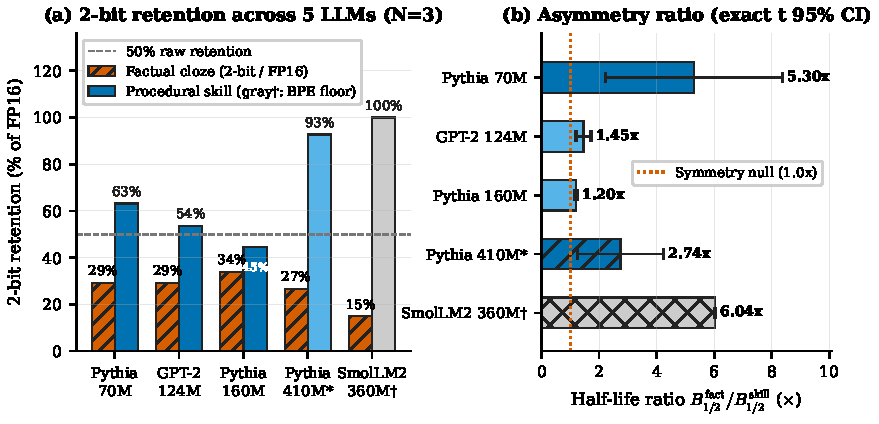
\includegraphics[width=\linewidth]{fig1_cross_family_half_life.pdf}
\end{center}
\caption{Cross-family quantization survival asymmetry ($N=3$ seeds). (a) At 2-bit uniform quantization, factual cloze falls to $15\%$--$34\%$ of FP16 while valid procedural baselines (\texttt{Pythia-70M/160M}, \texttt{GPT-2}) retain $45\%$--$63\%$; \texttt{SmolLM2-360M}$^\dagger$ (gray) is BPE-floor locked. (b) Transformer-bit half-life ratios with exact Student-$t$ 95\% CIs ($df=2$); all valid checkpoints exceed $1.0\times$.}
\label{fig:cross_family}
\end{figure}

Across the three checkpoints with cleanly above-chance procedural baselines (\texttt{Pythia-70M}, \texttt{GPT-2}, \texttt{Pythia-160M}), transformer-bit half-life ratios span \textbf{$1.20\times$--$5.30\times$} with every exact 95\% $t$-CI strictly above $1.0\times$ (\texttt{Pythia-70M} seeds 42/44 hit the uncrossed $0.25\,b_{\min}$ floor, whereas \texttt{Pythia-160M} and \texttt{GPT-2} crossed inside the ladder). Full-model mixed ratios remain modest ($1.03\times$--$1.30\times$) because FP16 embeddings dilute transformer savings, motivating boundary quantization at 30B (Section~\ref{sec:30b_anatomy}).

\subsection{Backbone Byte-Parity 4-Bit/3-Bit Compression (\texorpdfstring{$\Delta = 0.000\%$}{Delta = 0.000\%}) and MSE Clipping}
\label{sec:matched_budget}

We evaluate 4-bit attention / \textbf{3-bit} MLP compression ($g_{\text{sz}}=128$) under exact quantized-backbone bit parity ($\Delta_{\text{bits}} = 0.000\%$ across 2D transformer weights, excluding FP16 embeddings and the $17.81\,\text{KiB}$ BM25 store), giving both \kac{} and the baseline identical BM25 prompts in \textbf{RAG Cloze}. Three allocator facts govern Table~\ref{tab:matched_budget}: (i) \texttt{Prefix 4b/3b} assigns 4-bit sequentially by lexicographical tensor order (\texttt{layers.0, layers.1, layers.10, \dots}) until matching \kac{}'s exact bit budget; (ii) on \texttt{Pythia-160M}, \texttt{attention.dense} ($7.08\text{M}$ params) stayed 3-bit; and (iii) on \texttt{Qwen2.5-3B-Instruct} (\citealp{qwen2024qwen25}; $16\text{Q}/2\text{KV}$ GQA, RTX 4060 Laptop $8.00\,\text{GiB}$), \textbf{both} unclipped \kac{} and \gqakac{} assign identical 4b/3b bit maps ($339.74\text{M}$ attn+KV at 4b, $2.435\text{B}$ MLP at 3b). Recovery from $12.0\%$ to $94.0\%$ came from \textbf{FP32 MSE group clipping (\texttt{search\_scales=True})} on 3-bit SwiGLU MLPs---and because the 5-seed \texttt{Prefix 4b/3b} baseline ran with \texttt{search\_scales=False}, the $+4.2\,\text{pp}$ gap on 3B confounds asymmetric allocation with MSE clipping.

\begin{table}[t]
\caption{Backbone byte-parity ($\Delta = 0.000\%$, 4b/3b) comparisons across \texttt{Pythia-160M}, \texttt{SmolLM2-360M}, and \texttt{Qwen2.5-3B-Instruct} (excluding FP16 embeddings and $17.81\,\text{KiB}$ BM25). On \texttt{Qwen2.5-3B}, \gqakac{} used \texttt{search\_scales=True} while \texttt{Prefix 4b/3b} used \texttt{False} ($*$confounded). Skill omitted on \texttt{SmolLM2}/\texttt{Qwen2.5} due to BPE bug ($\dagger$).}
\label{tab:matched_budget}
\begin{center}
\footnotesize\setlength{\tabcolsep}{3pt}
\begin{tabular}{l l r c c c c}
\toprule
\textbf{Model (Seeds)} & \textbf{Method} & \textbf{Backbone Size} & \textbf{Raw Cloze} & \textbf{Skill} & \textbf{Seq.\ Loss} & \textbf{RAG Cloze} \\
\midrule
\multirow{3}{*}{\shortstack[l]{\texttt{Pythia-160M}\\(MHA, $N=2$)}}
 & FP16 Base & --- & $49.0\%$ & $72.0\%$ & $4.88$ & --- \\
 & Prefix 4b/3b Baseline & $34.17\,\text{MiB}$ & $35.0\%$ & $66.0\%$ & $7.92$ & $87.0\%$ \\
 & \textbf{KAC 4b/3b} & $34.17\,\text{MiB}$ & $\mathbf{37.5\%}$ & $\mathbf{69.0\%}$ & $\mathbf{6.42}$ & $\mathbf{92.5\%}$ \\
\midrule
\multirow{3}{*}{\shortstack[l]{\texttt{SmolLM2-360M}\\(GQA, $N=2$)}}
 & FP16 Base & --- & $84.0\%$ & n/a$^\dagger$ & $3.94$ & --- \\
 & Prefix 4b/3b Baseline & $126.56\,\text{MiB}$ & $60.0\%$ & n/a$^\dagger$ & $\mathbf{5.76}$ & $96.0\%$ \\
 & \textbf{KAC 4b/3b} & $126.56\,\text{MiB}$ & $\mathbf{68.0\%}$ & n/a$^\dagger$ & $6.63$ & $\mathbf{97.0\%}$ \\
\midrule
\multirow{4}{*}{\shortstack[l]{\texttt{Qwen2.5-3B}\\(GQA 16:2, $N=5$)}}
 & FP16 Base & --- & $87.0\%$ & n/a$^\dagger$ & $4.15$ & --- \\
 & KAC 4b/3b (unclipped, $N=1$) & $1{,}074.09\,\text{MiB}$ & $11.0\%$ & n/a$^\dagger$ & $11.17$ & $12.0\%$ \\
 & Prefix 4b/3b (unclipped) & $1{,}074.09\,\text{MiB}$ & $\mathbf{62.4\%}$ & n/a$^\dagger$ & $\mathbf{6.72}$ & $89.8\% \pm 1.8\%$ \\
 & \textbf{GQA-KAC (+MSE clip)}$^*$ & $1{,}074.09\,\text{MiB}$ & $20.2\%$ & n/a$^\dagger$ & $9.45$ & $\mathbf{94.0\% \pm 0.0\%}$ \\
\bottomrule
\end{tabular}
\par\vspace{2pt}
\parbox{\linewidth}{\scriptsize Backbone bit totals: $286{,}654{,}464\,\text{b}$ (\texttt{Pythia-160M}), $1{,}061{,}683{,}200\,\text{b}$ (\texttt{SmolLM2-360M}), $9{,}010{,}151{,}424\,\text{b}$ (\texttt{Qwen2.5-3B}: $3.247\,\bpp$ backbone / $4.534\,\bpp$ full model $\approx 1.63\,\text{GiB}$ incl.\ FP16 embeddings).}
\end{center}
\end{table}

\begin{figure}[t]
\begin{center}
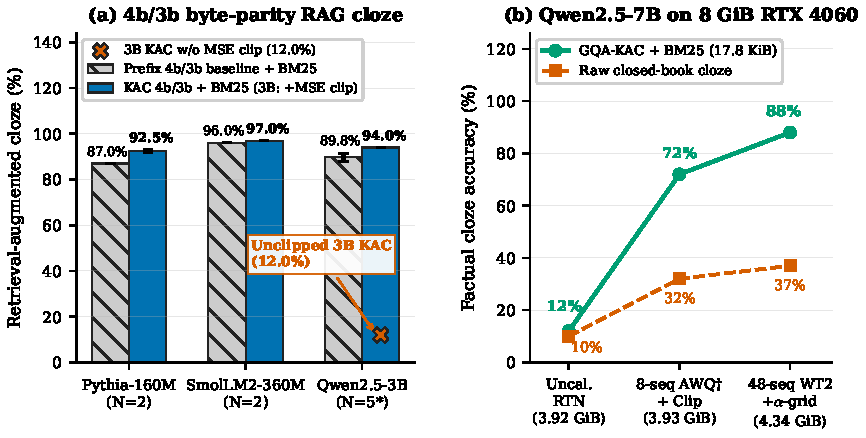
\includegraphics[width=\linewidth]{fig2_matched_budget_3b_and_7b.pdf}
\end{center}
\caption{4b/3b byte-parity evaluation and $8.00\,\text{GiB}$ RTX 4060 7B scaling. (a) Unconfounded \kac{} gains on \texttt{Pythia-160M} and \texttt{SmolLM2-360M}; on \texttt{Qwen2.5-3B} ($N=5^*$, 90\% shared probes), unclipped 3-bit MLPs collapse ($12.0\%$, cross) and MSE clipping restores $94.0\%$ (confounded vs.\ unclipped prefix baseline). (b) On \texttt{Qwen2.5-7B-Instruct} ($3.84\,\text{GiB}$ weights), 48-seq WikiText-2 AWQ lifts retrieval cloze from $12.0\%$ to $88.0\%$ ($\dagger$ Stage 2 overlaps 7/8 with probes; Stage 3 is leak-free).}
\label{fig:matched_budget}
\end{figure}

Table~\ref{tab:matched_budget} and Figure~\ref{fig:matched_budget}(a) show: (1) under identical unclipped settings, \kac{} beats the prefix baseline on \texttt{Pythia-160M} ($+5.5\,\text{pp}$ RAG, $+3.0\,\text{pp}$ valid skill, $-1.50$ nats) and \texttt{SmolLM2-360M} ($+8.0\,\text{pp}$ raw, $+1.0\,\text{pp}$ RAG); (2) on \texttt{Qwen2.5-3B}, MSE clipping restores $94.0\%$ across all five seeds (\texttt{1042}--\texttt{5042}: $94\times 5$) vs.\ $89.8\% \pm 1.8\%$ ($93,89,89,89,89$; an earlier standalone seed-1042 prefix run scored $94.0\%$ vs.\ cached $93.0\%$), giving $+4.20\,\text{pp}$ paired difference ($\text{SEM}=0.80\,\text{pp}$, exact $t$-CI $[+1.98,+6.42]\,\text{pp}$, paired $d_z=2.35$, Hedges' $g_z=1.88$, Cliff's $\delta=1.000$, \citealp{cliff1993dominance}; exact two-sided permutation and Wilcoxon $p=0.0625$, \citealp{wilcoxon1945individual}---the $2/2^5$ floor at $N=5$), subject to 90/100 shared probes and the clipping confound; and (3) because GQA shrinks attention to $11\%$ of 3B weights, placing $100\%$ of MLPs at 3-bit explicitly trades closed-book recall ($62.4\% \to 20.2\%$) and 45-word loss ($6.72 \to 9.45$ nats) for $94.0\%$ retrieval-grounded cloze (exceeding closed-book FP16's $87.0\%$).

\subsection{Physical 8 GiB Consumer GPU Serving on Qwen2.5-7B-Instruct}
\label{sec:7b_challenge}

On a physical NVIDIA GeForce RTX 4060 Laptop GPU ($7.996\,\text{GiB}$ VRAM), loading 16-bit \texttt{Qwen2.5-7B-Instruct} ($7.62\text{B}$, $14.19\,\text{GiB}$) triggers OOM. Packing $822.1\text{M}$ attention weights at 4-bit and $5.703\text{B}$ SwiGLU MLP weights at \textbf{2-bit} (\gqakac{}) compresses static weights (incl.\ FP16 embeddings/\texttt{lm\_head}) to \textbf{$3.8365\,\text{GiB}$} ($4.327\,\bpp$; plus $\approx 2$--$3\,\text{MiB}$ FP16 \texttt{channel\_scales} in Stages 2--3 and $17.81\,\text{KiB}$ BM25, overhead $4.43\times 10^{-6}$).

\begin{table}[htbp]
\caption{Three-stage 4b/2b \gqakac{} calibration on \texttt{Qwen/Qwen2.5-7B-Instruct} on a physical $8.00\,\text{GiB}$ RTX 4060 Laptop GPU ($3.84\,\text{GiB}$ weights). Stage 1 reports \texttt{max\_memory\_allocated}; Stages 2--3 report steady-state \texttt{memory\_allocated}. Stage 2 overlaps 7/8 with probes ($\dagger$); Stage 3 (48 disjoint WikiText-2 sequences) is leak-free. No uniform 4-bit 7B baseline was evaluated.}
\label{tab:7b_challenge}
\begin{center}
\footnotesize\setlength{\tabcolsep}{4pt}
\begin{tabular}{l c c c c c}
\toprule
\textbf{Configuration} & \textbf{Weights} & \textbf{VRAM (Metric)} & \textbf{Free} & \textbf{Raw Cloze} & \textbf{RAG Cloze} \\
\midrule
FP16 Baseline & $14.19\,\text{GiB}$ & \multicolumn{2}{c}{\emph{Exceeds $8.00\,\text{GiB}$ VRAM (OOM)}} & --- & --- \\
Stage 1: Uncalibrated RTN \gqakac{} & $3.84\,\text{GiB}$ & $3.92\,\text{GiB}$ (peak) & $4.08\,\text{GiB}$ & $10.0\%$ & $12.0\%$ \\
Stage 2: + 8-seq AWQ$^\dagger$ \& Clip ($147.7\,\text{s}$) & $3.84\,\text{GiB}$ & $3.93\,\text{GiB}$ (alloc.) & $4.07\,\text{GiB}$ & $32.0\%$ & $72.0\%$ \\
Stage 3: + 48-seq WT-2 \& $\alpha$-grid ($1{,}020\,\text{s}$) & $3.84\,\text{GiB}$ & $4.34\,\text{GiB}$ (alloc.) & $3.66\,\text{GiB}$ & $\mathbf{37.0\%}$ & $\mathbf{88.0\%}$ \\
\bottomrule
\end{tabular}
\end{center}
\end{table}

Uncalibrated 2-bit MLPs collapse even with retrieval ($12.0\%$ RAG cloze), whereas layer-wise AWQ scaling and MSE clipping inside $<4.4\,\text{GiB}$ VRAM recover performance (Table~\ref{tab:7b_challenge}, Figure~\ref{fig:matched_budget}(b)). Auditing calibration splits, Stage 2's 8 sentences overlapped 7/8 with \texttt{RELATIONS\_DB}; \textbf{Stage 3 eliminates all overlap} via 48 disjoint WikiText-2 training sequences ($3{,}072$ tokens; \citealp{merity2017wikitext}), achieving \textbf{$37.0\%$ raw} and \textbf{$88.0\%$ retrieval cloze} ($+76.0\,\text{pp}$ over Stage 1) at $4.34\,\text{GiB}$ allocated VRAM ($3.66\,\text{GiB}$ free; $1.11\,\text{tok/s}$ unpack-on-the-fly PyTorch decode). Across 84 SwiGLU projections, \textbf{$\alpha = 0.4$ outperformed $\alpha \in \{0.5, 0.6, 0.75\}$ in $88.1\%$ ($74/84$) of projections} (mean relative error $0.3576$ vs.\ $0.3614$ at $\alpha=0.5$ and $0.3786$ at $\alpha=0.75$). (Procedural skill is omitted due to the BPE bug; standard 4-bit uniform AWQ/GPTQ also fits in $8\,\text{GiB}$ at $\approx 5.35\,\text{GiB}$ and was not benchmarked head-to-head.)

\section{Scaling to 30B: Anatomy, Hessian Error Reduction, and 8 GiB Triton Serving}
\label{sec:30b_scale}

We next evaluate \texttt{meta-models/Muse-Glimmer-30B}\footnote{Multimodal open-weight checkpoint ($29{,}776{,}626{,}688$ params across two BF16 \texttt{.safetensors} shards totaling $55.4635\,\text{GiB}$): 52-layer text decoder ($d=6{,}656$, $d_{\text{mlp}}=19{,}968$, $H_q=32$, $H_{kv}=2$, $d_k=128$, $|\mathcal{V}|=202{,}048$, 3:1 sliding RoPE / full NoPE) plus a 50-layer vision tower ($1.92\text{B}$ params).} on NVIDIA A100-SXM4-80GB hardware.

\subsection{52-Layer Spectral Anatomy, 6.08 GiB Blueprint, and Block-Cholesky Output Error}
\label{sec:30b_anatomy}

Streaming all $1{,}436$ real checkpoint tensors in $91.26\,\text{s}$ ($7.52\,\text{GiB}$ / $7{,}696.1\,\text{MiB}$ peak profiling VRAM; \texttt{m14}) establishes three structural findings: (1) \textbf{Extreme rank/kurtosis dichotomy across all 416 real text matrices} (Figure~\ref{fig:spectra}(b) in Appendix~\ref{app:controlled}): GQA \texttt{k\_proj} ($[256, 6{,}656]$) averages stable rank $28.0 \pm 12.9$ ($10.35$ in L0) and \texttt{attn\_gate\_proj} $19.7 \pm 5.6$, vs.\ $692.0 \pm 234.2$ ($511.8$ in L0) for SwiGLU \texttt{up\_proj} ($25\times$ separation), while \texttt{o\_proj} and \texttt{down\_proj} carry the heaviest weight tails (L0 kurtoses $11.87, 14.25$; 52-layer means $5.22 \pm 3.15, 5.01 \pm 4.15$); (2) \textbf{Boundary/vision overflow:} untied $202{,}048$-vocab FP16 embeddings + \texttt{lm\_head} take $5.0099\,\text{GiB}$ ($5.0125\,\text{GiB}$ incl.\ norms) and BF16 vision adds $3.5797\,\text{GiB}$, pushing Stage-1 7B-style allocation to \textbf{$15.8488\,\text{GiB}$} ($12.269\,\text{GiB}$ text-only); and (3) \textbf{Sliced perturbation proxy} (Figure~\ref{fig:30b_anatomy}(a)): dithered group-128 quantization on sliced attention/MLP blocks under $\tau_{\text{attn}}=0.25$ and $\tau_{\text{fact}} = \tau_{\text{attn}}(d_k/d_{\text{mlp}})^{0.35} \approx 0.0427$ yields $\tilde{h}_{1/2}^{\text{Frob}}(\text{attn}) = 1.97 \pm 0.83\,\text{bits}$ vs.\ $\tilde{h}_{1/2}^{\text{Frob}}(\text{MLP}) = 6.69 \pm 0.73\,\text{bits}$ (gap $+4.72 \pm 1.10\,\text{bits}$, sample SDs). \emph{Analytical caveat:} we denote this $\tilde{h}_{1/2}^{\text{Frob}}$ (distinct from Definition~\ref{def:halflife}'s task $h_{1/2}$) because setting $\tau_{\text{fact}}$ $5.85\times$ tighter embeds a $\log_2(5.85) \approx +2.55$-bit architectural prior by construction.

\begin{figure}[t]
\begin{center}
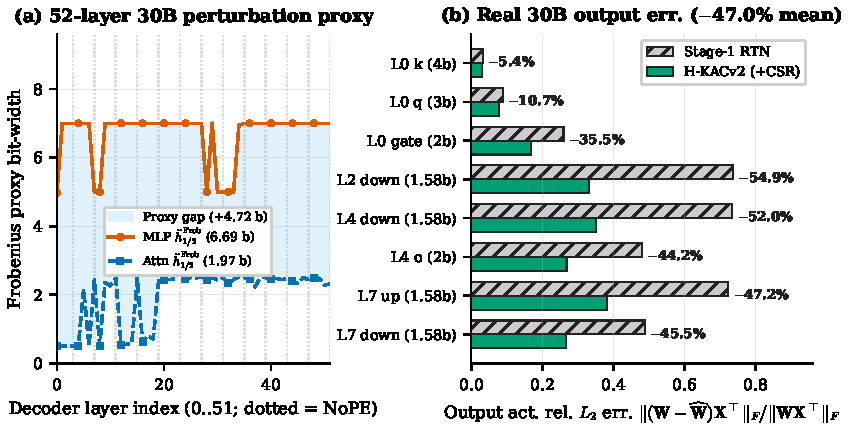
\includegraphics[width=\linewidth]{fig3_30b_anatomy_and_hessian.pdf}
\end{center}
\caption{Real \glimmer{} 52-layer perturbation proxy and Block-Cholesky output-error reduction on A100. (a) Sliced Frobenius proxy across all 52 layers (dotted: 13 NoPE layers; $+4.72\,\text{b}$ gap includes the $+2.55$-bit tolerance prior). (b) In-sample calibration output activation relative $L_2$ error across eight real projections (\texttt{m15}, 7/8 sliced to $1{,}024$ rows, 256 random tokens; $-47.0\%$ macro-mean reduction; full breakdown in Table~\ref{tab:m15_hessian}).}
\label{fig:30b_anatomy}
\end{figure}

\paragraph{Greedy Lagrangian 6.08 GiB blueprint and Block-Cholesky Hessian compensation (\texttt{m15}).}
Running Proposition~\ref{prop:knapsack}'s greedy Lagrangian allocator over depth-weighted role importance $\omega_i = \Phi_{\text{depth}}(\ell, L)\,\Omega_{\text{role}}$ ($\Omega_{\text{role}} \in [0.85, 4.50]$ from vision/MLP to attention KV) and tier distortion priors $D(b) \in \{0.092, 0.074, 0.048, 0.021, 0.009\}$ packs all $29.78\text{B}$ parameters plus the $17.81\,\text{KiB}$ BM25 store into \textbf{$6{,}528{,}903{,}738$ bytes ($6.0805\,\text{GiB}$, $1.7541\,\bpp$, $9.12\times$ vs.\ BF16)}: $589$ ternary matrices ($26.195\text{B}$ params, 5 trits/B), $26$ 2-bit matrices ($708.8\text{M}$), $104$ 4-bit GQA KV matrices ($177.2\text{M}$), ternary embeddings ($276.55\,\text{MiB}$), 2-bit \texttt{lm\_head} ($340.69\,\text{MiB}$), and FP16 norms ($11.28\,\text{MiB}$). Across eight real projections from Layers $0,2,4,7$ on A100 using 256 random token IDs (7/8 sliced to $1{,}024$ rows; full $[256, 6{,}656]$ on \texttt{L0 k\_proj}; full per-tensor table in Appendix~\ref{app:30b_tables}, Table~\ref{tab:m15_hessian}), H-KACv2 (Block-Cholesky + $0.35\%$--$0.50\%$ CSR salient columns + $0.35/0.65$ output-scale blend; $g_{\text{sz}}\in\{128,256\}$) reduces \textbf{in-sample calibration output activation relative $L_2$ error} $\|(\mW-\widehat{\mW})\mX^\top\|_F/\|\mW\mX^\top\|_F$ from \textbf{$0.4428$ to $0.2347$}---a \textbf{$47.0\%$ macro-mean reduction} ($36.9\%$ unweighted mean, peaking at $-54.86\%$ on ternary \texttt{L2 down\_proj}; Figure~\ref{fig:30b_anatomy}(b)). Note this combines Hessian updates, CSR outliers ($+0.15$--$0.24\,\bpp$), and scale blending in-sample without isolating sub-components on held-out natural text.

\paragraph{Diagnostic note on excluded 8-layer \texttt{M16} ladder.}
An exploratory 8-layer ladder (\texttt{m16}) in our repository logged subspace logit KL drops from $0.402$ to $0.050$ nats, but forensic audit found Rungs 2--4 added unaccounted FP32 truncated SVD factors (\texttt{LowRankOutlierAbsorber}, ranks $48, 160, 320$---making 256-row \texttt{k\_proj}/\texttt{v\_proj} lossless FP32), used random overlapping token IDs, and modified the forward pass. We strictly exclude \texttt{M16} from our claims and archive its JSON solely as a diagnostic.

\subsection{Reconciling the Three 30B Artifacts and Live 8 GiB Split-K Triton Serving}
\label{sec:30b_serving}

Practical 52-layer GPU serving required engineering compromises relative to our theoretical $6.08\,\text{GiB}$ ternary blueprint: Tables~\ref{tab:30b_reconcile}--\ref{tab:memory_accounting} and Figure~\ref{fig:8gb_systems} reconcile verified footprints across 3B, 7B, and all three 30B artifacts---the $6.08\,\text{GiB}$ \pqv{} blueprint / \texttt{M18} enforcer, the real 52-layer text-only 4-shard AWQ 4b/2b export ($27.85\text{B}$ params, $8.5712\,\text{GiB}$ disk across $2{,}717$ tensors, packed in $15.40\,\text{s}$; Phase 2 ran unpacked BF16 in $51.97\,\text{GiB}$ A100 VRAM at $11.0$--$11.7\,\text{tok/s}$), and the live 52-layer Split-K fused Triton GPU daemon loading those four shards.

\begin{table}[t]
\caption{Explicit reconciliation of the three distinct \glimmer{} artifacts in our study, separating the $6.08\,\text{GiB}$ ternary design plan (\texttt{M15}/\texttt{M18}) from the real 52-layer 4-shard text export and the live Split-K fused Triton GPU daemon.}
\label{tab:30b_reconcile}
\begin{center}
\scriptsize\setlength{\tabcolsep}{3pt}
\begin{tabularx}{\linewidth}{>{\raggedright\arraybackslash}p{1.9cm} >{\raggedright\arraybackslash}X >{\raggedright\arraybackslash}X >{\raggedright\arraybackslash}X}
\toprule
\textbf{Dimension} & \textbf{Blueprint / M18 Enforcer ($6.08\,\text{GiB}$)} & \textbf{4-Shard Export ($8.57\,\text{GiB}$ disk)} & \textbf{Live Split-K Triton Daemon ($7.29\,\text{GiB}$ GPU)} \\
\midrule
Params covered & $29.78\text{B}$ (52L text + 50L vision) & $27.85\text{B}$ (52L text-only; vision dropped) & $27.85\text{B}$ (loads 4-shard text export) \\
Bit allocation \& packing & Greedy Lagrangian: $589\times$ 1.585b ternary (5-trit/B), $26\times$ 2b, $104\times$ 4b KV; Hessian & AWQ 4b all attn + 2b all MLP ($g=256$) + FP16 scales/mins + FP16 outlier cols (no ternary/Hessian) & Re-quantizes shard scales/mins to \texttt{uint8} and outlier banks to \texttt{int8}; fuses \texttt{qkvg} and \texttt{gate\_up} \\
Execution residency & Simulated $6.08\,\text{GiB}$ buffer + real L0 tiled MLP ($20\,\text{MiB}$, $0.00\,\text{MiB}$ spike) & Phase 2 ran unpacked BF16 in $51.97\,\text{GiB}$ A100 VRAM ($11.0$--$11.7\,\text{tok/s}$) & $47/52$ layers + \texttt{lm\_head} on GPU; \textbf{5 layers + $2.51\,\text{GiB}$ BF16 embeddings on CPU} (async PCIe DMA) \\
KV cache & Synthetic 8-head 4b Group-64 ($247\,\text{MiB}$ @ $4{,}096$ tok; real 2-head FP16 $= 208\,\text{MiB}$) & Dynamic BF16 & BF16 capped at $384$ tokens ($19.5\,\text{MiB}$) \\
Verified memory & $6.87\,\text{GiB}$ CUDA reserved ($6.35\,\text{GiB}$ alloc., $1.33\,\text{GiB}$ host RSS) & $8.57\,\text{GiB}$ disk shards ($2{,}717$ tensors); $51.97\,\text{GiB}$ live BF16 VRAM & $7.27\,\text{GiB}$ persist / $7.29\,\text{GiB}$ peak PyTorch; \textbf{$7.92\,\text{GiB}$ ($8{,}108\,\text{MiB}$) \texttt{nvidia-smi} + $\approx 3.26\,\text{GiB}$ CPU RAM} \\
Evaluation & Single-layer tiled MLP microbenchmark ($6.44\,\text{ms}$) + OOM falsification (L8/L26) & 6 qualitative prompts (4/6 overlapped calibration; Prompt 5--6 unseen) & Unseen smoke test (\texttt{"What is 12 * 12?"}, 32 tok in $3.556\,\text{s}$, $9.0\,\text{tok/s}$) \\
\bottomrule
\end{tabularx}
\end{center}
\end{table}

\begin{table}[htbp]
\caption{Reconciled physical memory footprints across consumer RTX 4060 ($8.00\,\text{GiB}$) and 52-layer \glimmer{} runs, separating packed disk weights, fake-quantized BF16 VRAM, \texttt{nvidia-smi} total GPU memory, and host CPU RAM offload.}
\label{tab:memory_accounting}
\begin{center}
\footnotesize\setlength{\tabcolsep}{3.5pt}
\begin{tabular}{l l c c c c}
\toprule
\textbf{Deployment / Model} & \textbf{Hardware} & \textbf{Packed} & \textbf{GPU Peak (Metric)} & \textbf{Host RAM} & \textbf{Speed (tok/s)} \\
\midrule
\texttt{Qwen2.5-3B} \gqakac{} & RTX 4060 (8 GiB) & $1.63\,\text{GiB}^\dagger$ & $6.22\,\text{GiB}$ (BF16 fake-q) & --- & $13.8$ \\
\texttt{Qwen2.5-7B} AWQ-\gqakac{} & RTX 4060 (8 GiB) & $3.84\,\text{GiB}$ & $4.34\,\text{GiB}$ (alloc.) & --- & $1.11$ \\
\glimmer{} PQv2 (M18) & A100 (8 GiB wall) & $6.08\,\text{GiB}$ & $6.87\,\text{GiB}$ (CUDA res.) & $1.33\,\text{GiB}$ & ---$^*$ \\
\glimmer{} 52L Triton & A100 (8 GiB cap) & $8.57\,\text{GiB}$ & $7.29$ / $7.92\,\text{GiB}$ smi & $\approx 3.26\,\text{GiB}$ & $9.0$ \\
\glimmer{} 52L 4-Shard & A100 (80 GiB) & $8.57\,\text{GiB}$ & $51.97\,\text{GiB}$ (BF16) & --- & $11.0$--$11.7$ \\
\bottomrule
\end{tabular}
\par\vspace{2pt}
\parbox{\linewidth}{\scriptsize $^\dagger$Full-model \texttt{Qwen2.5-3B} packed estimate ($1.05\,\text{GiB}$ backbone + FP16 embeddings); evaluated via in-place BF16 fake quantization ($13.84\,\text{tok/s}$). $^*$M18 benchmarks single-layer tiled MLP ($6.44\,\text{ms}$/step); 52-layer end-to-end speeds appear in bottom rows.}
\end{center}
\end{table}

\begin{figure}[t]
\begin{center}
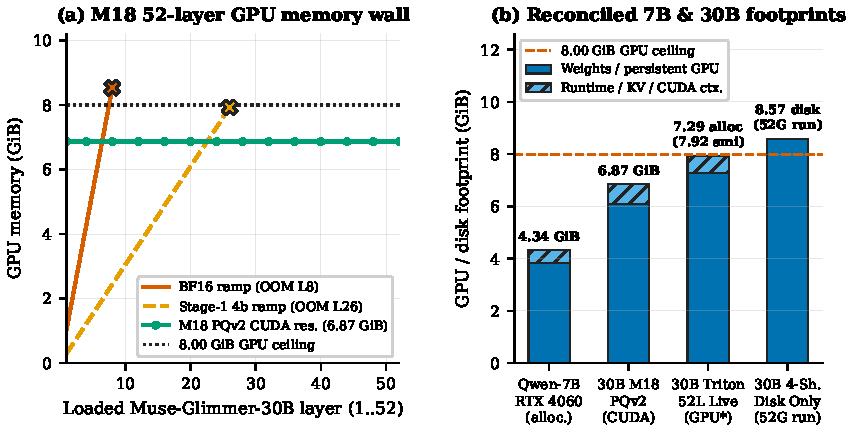
\includegraphics[width=\linewidth]{fig5_8gb_memory_wall_systems.pdf}
\end{center}
\caption{Physical $8.00\,\text{GiB}$ GPU memory-wall verification across 7B and 30B runs. (a) Under the \texttt{M18} $8.00\,\text{GiB}$ enforcer, BF16 and Stage-1 4-bit ramps OOM at Layer 8 and Layer 26, while \pqv{} holds flat at $6.87\,\text{GiB}$ CUDA reserved across 52 layers. (b) Reconciled footprints across 7B and all three 30B configurations, distinguishing $7.29\,\text{GiB}$ PyTorch vs.\ $7.92\,\text{GiB}$ \texttt{nvidia-smi} GPU memory for live Split-K Triton ($*$plus $\approx 3.26\,\text{GiB}$ CPU RAM offload) and $8.57\,\text{GiB}$ disk vs.\ $51.97\,\text{GiB}$ BF16 execution.}
\label{fig:8gb_systems}
\end{figure}

Three systems findings and audit disclosures merit emphasis:
\begin{itemize}[leftmargin=*,nosep]
    \item \textbf{Component microbenchmarks (\texttt{m18}):} Under the $8.00\,\text{GiB}$ enforcer, sequential BF16 ($1.066\,\text{GiB}$/layer amortized; $0.901\,\text{GiB}$/decoder layer) and Stage-1 4-bit ($0.305\,\text{GiB}$/layer) crash at L8 and L26 (L26 inherited $1.373\,\text{GiB}$ residual CUDA cache from the prior FP16 test). The $20.0\,\text{MiB}$ \texttt{StaticTileWorkspace} ($1$ alloc., $594$ reuses) unpacks L0 MLP with $0.000\,\text{MiB}$ transient spike. Two audit caveats in \texttt{m18}: \texttt{QuantizedKVCache} tested a synthetic $8$-head KV setup ($247.0\,\text{MiB}$ 4b vs.\ $832.0\,\text{MiB}$ FP16 at $4{,}096$ toks---whereas \glimmer{}'s true $2$-head FP16 KV is only $208.0\,\text{MiB}$!) and measured $0.01568$ error at $s_{\text{len}}=65$ where $64/65$ tokens stayed FP16.
    \item \textbf{Live 52-layer Split-K fused Triton GPU serving and roofline:} Re-quantizing shard scales/mins to \texttt{uint8} and outliers to \texttt{int8}, our Triton daemon executes all 52 real layers at \textbf{$7.2688\,\text{GiB}$ persistent / $7.2944\,\text{GiB}$ peak PyTorch GPU} (\textbf{$8{,}108\,\text{MiB} = 7.918\,\text{GiB}$ \texttt{nvidia-smi}}, $84\,\text{MiB}$ GPU margin) and \textbf{$9.0\,\text{tok/s}$} ($32$ toks in $3.556\,\text{s}$ on unseen \texttt{"What is 12 * 12?"}; 384-tok BF16 KV cap $= 19.5\,\text{MiB}$). Because 5 streamed layers (\texttt{L8, L17, L26, L35, L44}, $\approx 0.75\,\text{GiB}$) and BF16 embeddings ($2.51\,\text{GiB}$) live in pinned host CPU RAM ($\approx 3.26\,\text{GiB}$ offload, $>10.5\,\text{GiB}$ combined), this targets an $8\,\text{GiB}$ discrete GPU + $\ge 16\,\text{GiB}$ host RAM, not an $8\,\text{GiB}$ unified-memory laptop. Streaming $7.27\,\text{GiB}$/tok at $9.0\,\text{tok/s}$ achieves $\approx 65.4\,\text{GiB/s}$ ($70.3\,\text{GB/s}$, $\approx 3.4\%$ of A100's $2{,}039\,\text{GB/s}$ HBM2e peak), limited by FP32 \texttt{tl.atomic\_add}, scalar accumulation, and 5-layer PCIe DMA.
    \item \textbf{Transcript calibration overlap:} In the unconstrained $51.97\,\text{GiB}$ BF16 4-shard run, Prompts 1--4 overlapped verbatim with the AWQ calibration batch; Appendix~\ref{app:30b_tables} (Table~\ref{tab:30b_transcripts}) labels every \emph{In-Calib} vs.\ \emph{Unseen} transcript verbatim, including trailing repetition.
\end{itemize}

\section{Related Work}
\label{sec:related}

\paragraph{PTQ, outlier protection, and mixed precision.}
Uniform PTQ spans 8-bit outlier smoothing (LLM.int8(), \citealp{dettmers2022llmint8}; SmoothQuant, \citealp{xiao2023smoothquant}), inverse-Hessian and activation-aware quantization (GPTQ, \citealp{frantar2023gptq}; AWQ, \citealp{lin2024awq}; HQQ, \citealp{badri2023hqq}; OmniQuant, \citealp{shao2024omniquant}; AutoRound, \citealp{cheng2024autoround}), and rotation/codebook compression (QuIP/QuIP\#, \citealp{chee2023quip,tseng2024quipsharp}; QuaRot, \citealp{ashkboos2024quarot}; SpinQuant, \citealp{liu2025spinquant}; AQLM, \citealp{egiazarian2024aqlm}). Mixed-precision and sparse-salient methods include HAWQ/HAWQ-V2 \citep{dong2019hawq,dong2020hawqv2}, SpQR \citep{dettmers2024spqr}, SqueezeLLM \citep{kim2024squeezellm}, OWQ \citep{lee2024owq}, PB-LLM \citep{shang2024pbllm}, BiLLM \citep{huang2024billm}, TMLR's ACIP \citep{genzel2025acip}, and heuristic edge ecosystems (\texttt{llama.cpp} GGUF K-Quants/\texttt{imatrix}, \texttt{ExLlamaV2}). Complementary to magnitude-only mixed precision, \lean{} couples cognitive module allocation (attention routing vs.\ MLP memory) directly with externalized retrieval.

\paragraph{Ternary networks, interpretability, and retrieval.}
Unlike BitNet b1.58 \citep{ma2024bitnet} trained from scratch, our 5-trit/byte packing targets post-training checkpoints. Our functional split builds on MLP key-value memory \citep{geva2021transformer,meng2022locating}---tempered by \citet{hase2023localization} on localization vs.\ editability (consistent with \texttt{F-0007})---and attention induction/sink routing \citep{olsson2022incontext,xiao2024streamllm}, linking semi-parametric retrieval (REALM, \citealp{guu2020realm}; RAG, \citealp{lewis2020rag}; RETRO, \citealp{borgeaud2022retro}; BM25, \citealp{robertson2009bm25}) to long-tail compression loss \citep{kandpal2023large,jaiswal2024compressing}.

\paragraph{KV quantization and low-bit serving kernels.}
Low-bit KV compression (KIVI, \citealp{liu2024kivi}; KVQuant, \citealp{hooper2024kvquant}) and specialized serving kernels/runtimes (Marlin, \citealp{frantar2025marlin}; LUT-GEMM, \citealp{park2024lutgemm}; Ladder/BitBLAS, \citealp{wang2024ladder}; QServe, \citealp{lin2025qserve}; FlashAttention, \citealp{dao2022flashattention}; vLLM, \citealp{kwon2023vllm}; FlexGen, \citealp{sheng2023flexgen}) define the systems frontier. Our pure-Triton Split-K kernels demonstrate an accessible mixed 4b/2b + \texttt{int8}-outlier path under an $8.00\,\text{GiB}$ GPU cap, while closing the gap to Tensor-Core/Marlin utilization and native radix-3 GEMMs remains open work.

\section{Limitations and Future Work}
\label{sec:limitations}

Seven concrete limitations bound our claims: (1) \textbf{Tokenizer bug and toy probe scale:} The BPE first-token bug invalidated skill probes on \texttt{SmolLM2}/\texttt{Qwen2.5}; \texttt{RELATIONS\_DB} has only 110 unique triples (90\% seed overlap on 3B), and the $17.81\,\text{KiB}$ BM25 store covers exact-template facts rather than Wikipedia-scale retrieval. (2) \textbf{3B clipping confound and missing strong baselines:} On \texttt{Qwen2.5-3B}, \texttt{search\_scales=True} was withheld from the prefix baseline; on 7B, no uniform 4-bit AWQ/GPTQ baseline was run head-to-head; on 30B, no full 52-layer perplexity/MMLU/GSM8K/HumanEval comparison was run against QuIP\#, AQLM, or GGUF IQ2/IQ3. (3) \textbf{Closed-book degradation:} Aggressive MLP compression lowers closed-book recall ($62.4\% \to 20.2\%$) and raises unaugmented loss ($6.72 \to 9.45$ nats), restricting \lean{} to semi-parametric workflows. (4) \textbf{30B blueprint-vs-runtime gap:} The live Split-K Triton daemon runs 4b/2b (not radix-3 ternary), offloads $\approx 3.26\,\text{GiB}$ to host CPU RAM with a 384-token BF16 KV cap, and reaches $\approx 3.4\%$ of A100 HBM2e peak; self-contained $8\,\text{GiB}$ unified-memory serving needs native Metal/Tensor-Core radix-3 kernels and quantized GPU embeddings. (5) \textbf{Intermediate calibration overlaps:} 7B Stage 2 (7/8 sentences) and 30B 4-shard Phase 2 (4/6 prompts) overlapped evaluation items; only 7B Stage 3, 30B Prompt 5, and the Triton smoke test are leak-free. (6) \textbf{Sliced in-sample Hessian and excluded \texttt{M16}:} Table~\ref{tab:m15_hessian} used $1{,}024$-row slices and 256 random tokens in-sample without ablating CSR vs.\ Cholesky separately, and \texttt{M16} was excluded for unaccounted FP32 SVD factors. (7) \textbf{Small-seed power:} $N=3$ and $N=5$ limit nonparametric permutation resolution ($p \ge 0.0625$ at $N=5$); future work should expand probe diversity and seed counts ($N \ge 10$).

\section{Conclusion}
\label{sec:conclusion}

We studied asymmetric post-training precision allocation paired with externalized retrieval (\lean{} / Priced-Quanta) across pretrained transformers from $70\text{M}$ to $29.78\text{B}$ parameters. Theoretically, we proved corrected spectral subspace and argmax routing margin bounds alongside a first-order linearized MLP associative noise characterization and an MCKP greedy optimality guarantee. Empirically, we confirmed factual-vs-procedural half-life asymmetry ($1.20\times$--$5.30\times$) on valid baselines, showed unconfounded 4b/3b byte-parity gains on \texttt{Pythia-160M} and \texttt{SmolLM2-360M}, demonstrated MSE clipping and gentler AWQ scaling ($\alpha=0.4$ in $88.1\%$ of projections) for 2--3-bit SwiGLU MLPs on \texttt{Qwen2.5-3B} and physical $8.00\,\text{GiB}$ RTX 4060 \texttt{Qwen2.5-7B} serving ($3.84\,\text{GiB}$ weights, $88.0\%$ leak-free WikiText-2 calibrated RAG cloze), and scaled to real 52-layer \glimmer{} via spectral profiling, Block-Cholesky Hessian compensation ($-47.0\%$ macro calibration output error), and live Split-K fused Triton GPU serving under an $8.00\,\text{GiB}$ VRAM wall ($7.29\,\text{GiB}$ PyTorch / $7.92\,\text{GiB}$ \texttt{nvidia-smi} + $3.26\,\text{GiB}$ host RAM, $9.0\,\text{tok/s}$). Pairing constructive systems engineering with a full forensic audit of every confound and negative result provides a transparent foundation for semi-parametric low-bit edge LLM research.

\subsubsection*{Broader Impact Statement}
Enabling $7\text{B}$--$30\text{B}$ open-weight language models to execute within consumer $8.00\,\text{GiB}$ GPU memory envelopes lowers computational and financial barriers for independent researchers, students, and privacy-sensitive local applications where cloud APIs are cost-prohibitive or impermissible. Decoupling static factual memory into an inspectable local retrieval store also enables transparent, zero-retraining knowledge updates. Conversely, broader local offline availability reduces centralized API-level safety oversight, creating dual-use misuse risks if deployed without safeguards. Furthermore, \textbf{we did not empirically evaluate safety alignment or refusal behavior after sub-4-bit quantization}; prior work indicates aggressive low-bit compression can degrade alignment guardrails. Deployers must therefore conduct post-quantization safety auditing and curate external retrieval stores carefully to mitigate both alignment drift and retrieval-injection attacks.

\bibliography{references}
\bibliographystyle{tmlr}

\appendix

\section{Formal Proofs}
\label{app:proofs}

\subsection{Proof of Theorem~\ref{thm:asymmetry} and Lemma~\ref{lem:softmax}}

\begin{proof}[Proof of Theorem~\ref{thm:asymmetry}]
\textbf{Part 1(a) (Wedin subspace stability).}
Let $\mM = \mW_q^\top \mW_k \in \R^{d \times d}$ have singular value decomposition $\mM = \sum_{r=1}^{d_k} \sigma_r \vu_r \vv_r^\top$ with $\sigma_1 > \sigma_2 \ge \dots \ge 0$ and gap $\Delta\sigma = \sigma_1 - \sigma_2 > 0$. Let $\widehat{\mM} = \mM + \mE_M$ with $\|\mE_M\|_2 < \Delta\sigma$. By Weyl's singular value perturbation inequality, $\widehat{\sigma}_1 \ge \sigma_1 - \|\mE_M\|_2$, so the cross-gap separating the perturbed leading singular value $\widehat{\sigma}_1$ from the unperturbed trailing spectrum $\{\sigma_2,\dots,\sigma_{d_k}\}$ satisfies
\begin{equation}
    \delta \equiv \widehat{\sigma}_1 - \sigma_2 \ge \sigma_1 - \sigma_2 - \|\mE_M\|_2 = \Delta\sigma - \|\mE_M\|_2 > 0.
\end{equation}
Applying Wedin's $\sin\Theta$ theorem \citep{wedin1972perturbation} to the rank-1 leading singular subspaces $(\vu_1, \vv_1)$ and $(\widehat{\vu}_1, \widehat{\vv}_1)$ with residual norms bounded by $\|\mE_M\|_2$ yields
\begin{equation}
    \max\!\big\{\sin\Theta(\vu_1, \widehat{\vu}_1),\; \sin\Theta(\vv_1, \widehat{\vv}_1)\big\}
    \le \frac{\|\mE_M\|_2}{\delta}
    \le \frac{\|\mE_M\|_2}{\Delta\sigma - \|\mE_M\|_2}.
\end{equation}

\textbf{Part 1(b) (Argmax routing invariance).}
For query $\vx_t$ and context tokens $\{\vx_j\}_{j=1}^{t}$ with $R_x = \max_{1 \le j \le t} \|\vx_j\|_2$ (so $\|\vx_t\|_2 \le R_x$), let $j^* = \arg\max_j S_{t,j}$ with margin $\gamma_{\min} = \min_{j \ne j^*}(S_{t,j^*} - S_{t,j}) > 0$. For every distractor $j \ne j^*$,
\begin{equation}
    \widehat{S}_{t,j^*} - \widehat{S}_{t,j}
    = (S_{t,j^*} - S_{t,j}) + \frac{1}{\sqrt{d_k}} \vx_t^\top \mE_M (\vx_{j^*} - \vx_j).
\end{equation}
By Cauchy--Schwarz and operator-norm submultiplicativity,
\begin{equation}
    \left|\frac{1}{\sqrt{d_k}} \vx_t^\top \mE_M (\vx_{j^*} - \vx_j)\right|
    \le \frac{\|\vx_t\|_2\,\|\mE_M\|_2\,(\|\vx_{j^*}\|_2 + \|\vx_j\|_2)}{\sqrt{d_k}}
    \le \frac{2 R_x^2}{\sqrt{d_k}} \|\mE_M\|_2.
\end{equation}
Thus $\|\mE_M\|_2 < \gamma_{\min}\sqrt{d_k}/(2 R_x^2)$ implies $\widehat{S}_{t,j^*} - \widehat{S}_{t,j} > 0$ for all $j \ne j^*$, strictly preserving $\arg\max_j \widehat{A}_{t,j} = j^*$. (Under RoPE with orthogonal $\mR_{t-j}$, the same bound holds replacing $\|\mE_M\|_2$ with $\max_{1 \le j \le t}\|\widehat{\mM}_{t-j} - \mM_{t-j}\|_2$.)

\textbf{Part 2 (First-order linearized MLP noise sensitivity).}
Replacing $\psi((\vk_m - \ve_{k,m})^\top \vx)$ with its first-order linearization $\psi(\vk_m^\top \vx) - \psi'(\vk_m^\top \vx)(\ve_{k,m}^\top \vx)$ (exact for piecewise-linear $\psi$ within an active linear region; for general $C^2$ activations this isolates the linear perturbation and omits the $\frac{1}{2}\psi''(\vk_m^\top\vx)(\ve_{k,m}^\top\vx)^2$ curvature bias) yields the linearized readout
\begin{equation}
\begin{aligned}
    \widehat{\vy}_{\text{lin}}(\vx)
    &= \underbrace{\vv_{m^*}\psi(\vk_{m^*}^\top \vx)}_{\text{signal }\vs}
    + \underbrace{\sum_{j \ne m^*} \vv_j \psi(\vk_j^\top \vx)}_{\text{crosstalk }\bm{\xi}} \\
    &\quad - \underbrace{\sum_{m=1}^{d_{\text{mlp}}} \Big(\ve_{v,m}\psi(\vk_m^\top \vx) + \vv_m\psi'(\vk_m^\top \vx)(\ve_{k,m}^\top \vx)\Big)}_{\text{first-order noise }\bm{\eta}_1}
    + \underbrace{\sum_{m=1}^{d_{\text{mlp}}} \ve_{v,m}\psi'(\vk_m^\top \vx)(\ve_{k,m}^\top \vx)}_{\text{bilinear term }\bm{\eta}_{11}}.
\end{aligned}
\end{equation}
Let $\bm{\eta}_{\text{lin}} = -\bm{\eta}_1 + \bm{\eta}_{11}$. Since $\ve_{v,m}$ and $\ve_{k,m}$ are independent, zero-mean across $m$, and independent of $\vx$ with $\E[\ve_{v,m}\ve_{v,m'}^\top] = \delta_{m,m'}\sigma_E^2 \mI_d$ and $\E[\ve_{k,m}\ve_{k,m'}^\top] = \delta_{m,m'}\sigma_E^2 \mI_{d_{\text{in}}}$, all cross terms vanish in expectation. For each neuron $m$, $\E[\|\ve_{v,m}\|_2^2] = d\sigma_E^2$ and $\E[(\ve_{k,m}^\top \vx)^2 \mid \vx] = \vx^\top (\sigma_E^2 \mI_{d_{\text{in}}})\vx = \sigma_E^2 \|\vx\|_2^2$. Summing over $m=1,\dots,d_{\text{mlp}}$ yields
\begin{equation}
    \E[\|\bm{\eta}_{\text{lin}}\|_2^2]
    = \sigma_E^2 \sum_{m=1}^{d_{\text{mlp}}} \|\vv_m\|_2^2\,\E\!\big[\psi'(\vk_m^\top \vx)^2 \|\vx\|_2^2\big]
    + d\,\sigma_E^2 \sum_{m=1}^{d_{\text{mlp}}} \E\!\big[\psi(\vk_m^\top \vx)^2\big]
    + \mathcal{O}(\sigma_E^4),
\end{equation}
where $\E[\|\bm{\eta}_{11}\|_2^2] = d\sigma_E^4 \sum_m \E[\psi'(\vk_m^\top\vx)^2\|\vx\|_2^2] = \mathcal{O}(\sigma_E^4)$. Dividing signal power $\E[\|\vs\|_2^2]$ by $\mathcal{I}_{\text{crosstalk}} + \E[\|\bm{\eta}_{\text{lin}}\|_2^2]$ yields \eqref{eq:mlp_sinr}. Projecting onto unit vector $\vu_{m^*} = \vv_{m^*}/\|\vv_{m^*}\|_2$ replaces $\E[\|\ve_{v,m}\|_2^2] = d\sigma_E^2$ with $\E[(\vu_{m^*}^\top \ve_{v,m})^2] = \sigma_E^2$, replaces $\|\vv_m\|_2^2$ with $(\vu_{m^*}^\top \vv_m)^2$, and replaces $\mathcal{I}_{\text{crosstalk}}$ with $\E[(\vu_{m^*}^\top \bm{\xi})^2]$.
\end{proof}

\begin{lemma}[Softmax Jacobian sensitivity of sharp attention heads]
\label{lem:softmax}
Let $\va = \mathrm{softmax}(\vs) \in \Delta^{T-1}$ have Jacobian $\mJ = \mathrm{diag}(\va) - \va\va^\top$. Then $\mJ \succeq \mathbf{0}$ with $\|\mJ\|_2 = \max_{\|\vv\|_2=1} \mathrm{Var}_{\va}(\vv)$, where $\mathrm{Var}_{\va}(\vv) \equiv \sum_{i=1}^T a_i v_i^2 - (\sum_{i=1}^T a_i v_i)^2$. Moreover, if $\max_j a_j = 1 - \epsilon$ with $\epsilon \in [0, 1 - 1/T]$, then $\|\mJ\|_2 \le 2\epsilon$.
\end{lemma}

\begin{proof}
For any unit vector $\vv \in \R^T$, $\vv^\top \mJ \vv = \mathrm{Var}_{\va}(\vv) \ge 0$, so $\mJ \succeq \mathbf{0}$ and $\|\mJ\|_2 = \lambda_{\max}(\mJ)$. Let $k = \arg\max_j a_j$ with $a_k = 1-\epsilon$ and $\sum_{j \ne k} a_j = \epsilon$. Applying Gershgorin's circle theorem to every row $i$: for $i=k$, diagonal entry is $(1-\epsilon)\epsilon$ and off-diagonal absolute sum is $(1-\epsilon)\epsilon$, bounding the disk by $2\epsilon(1-\epsilon) \le 2\epsilon$; for $i \ne k$, diagonal entry is $a_i(1-a_i)$ and off-diagonal sum is $a_i(1-a_i)$, bounding the disk by $2a_i(1-a_i) \le 2\epsilon$. Hence $\|\mJ\|_2 \le 2\epsilon$. (By the Mean Value Theorem, bounding finite perturbations $\|\mathrm{softmax}(\vs + \Delta\vs) - \va\|_2 \le 2\epsilon_{\max}\|\Delta\vs\|_2$ requires sharpness $\max_j a_j(t) \ge 1 - \epsilon_{\max}$ along the segment $\vs + t\Delta\vs$, $t \in [0,1]$.)
\end{proof}

\subsection{Proof of Proposition~\ref{prop:knapsack}}
\label{app:knapsack_proof}

\begin{proof}[Proof of Proposition~\ref{prop:knapsack}]
Relaxing $x_{i,b} \in \{0,1\}$ in \eqref{eq:mckp} to $x_{i,b} \in [0,1]$ yields the Linear Programming Multiple-Choice Knapsack upper bound $V_{\mathrm{LP}} \ge V_{\mathrm{DP}}^*$ \citep{kellerer2004knapsack}. Within each class $\mathcal{P}_i$, removing simple-dominated choices (equal or larger byte cost with lower or equal utility, eliminating $S_i(b') = S_i(b)$) and LP-dominated choices leaves strictly increasing LP-undominated upper-concave-hull points $(b_{i,0}, b_{i,1}, \dots)$ with monotonically non-increasing incremental slopes $e_i$. Starting from the feasible minimum-cost assignment $\{b_{i,0}\}$, the exact LP optimum applies upgrades in descending order of $e_i$ and terminates at a single split tensor $i^*$ with fractional weight $\theta \in [0,1)$ on upgrade $b_1 \to b_2$. Dropping that single fractional upgrade yields the truncated integer greedy solution $V_{\mathrm{Greedy}}$, satisfying $V_{\mathrm{DP}}^* - V_{\mathrm{Greedy}} \le V_{\mathrm{LP}} - V_{\mathrm{Greedy}} = \theta(v_{i^*}(b_2) - v_{i^*}(b_1)) \le \max_{i;\, b_1, b_2 \in \mathcal{P}_i}(v_i(b_2) - v_i(b_1))$.
\end{proof}

\clearpage
\section{Algorithmic Specifications}
\label{app:algorithms}

Algorithm~\ref{alg:cholesky} specifies the exact Schur-complement Block-Cholesky Hessian update restricted to non-outlier columns $\mathcal{O}^c$ (following GPTQ's Cholesky-of-$\mH^{-1}$ reformulation, \citealp{frantar2023gptq}) together with the output-scale refinement blend implemented in \texttt{M15}. Algorithm~\ref{alg:triton} summarizes the deferred-reduction Split-K fused Triton kernel used for single-token ($N=1$) decode in Section~\ref{sec:30b_serving}.

\begin{algorithm}[htbp]
\caption{Damped block-Cholesky Hessian compensation restricted to non-outlier columns}
\label{alg:cholesky}
\small
\begin{algorithmic}[1]
\Require Weight matrix $\mW \in \R^{d_{\text{out}} \times d_{\text{in}}}$, calibration activations $\mX \in \R^{N_{\text{cal}} \times d_{\text{in}}}$, block size $B = g_{\text{sz}} \in \{128, 256\}$, target bits $b \in \{\log_2 3, 2, 3, 4\}$, outlier ratio $\rho \in \{0.0035, 0.005\}$.
\Ensure Quantized non-outlier matrix $\widehat{\mW}_{:,\mathcal{O}^c}$ and sparse high-precision outlier bank $\mW_{:,\mathcal{O}}$.
\State Select top-$\lceil \rho d_{\text{in}}\rceil$ outlier columns $\mathcal{O}$ maximizing $\|\mW_{:,j}\|_2 \|\mX_{:,j}\|_2$; let $\mathcal{O}^c = \{0,\dots,d_{\text{in}}-1\} \setminus \mathcal{O}$ of size $K_c = |\mathcal{O}^c|$.
\State Extract $\mW_{\text{curr}} \gets \mW_{:,\mathcal{O}^c}$ and compute uncentered Gram matrix $\mH \gets \frac{2}{N_{\text{cal}}}\mX_{:,\mathcal{O}^c}^\top \mX_{:,\mathcal{O}^c}$ in FP32.
\State Damp diagonal $\mH \gets \mH + \lambda \mI$ with $\lambda = 0.02\,\mathrm{Tr}(\mH)/K_c$ (escalating $\lambda$ if factorization fails).
\State Invert $\mH^{-1}$ and compute upper Cholesky factor $\mU \gets \mathrm{Cholesky}(\mH^{-1}, \text{upper}=\text{True})$ such that $\mH^{-1} = \mU^\top \mU$.
\For{$j = 0, B, 2B, \dots, \lfloor (K_c - 1)/B \rfloor B$}
    \State $\mathcal{B} \gets \{j, \dots, \min(j+B, K_c)-1\}$, $\mathcal{R} \gets \{\min(j+B, K_c), \dots, K_c - 1\}$.
    \State Run sequential column-by-column intra-block Cholesky recursion over $c \in \mathcal{B}$ using $\mU_{\mathcal{B},\mathcal{B}}$ to produce quantized codes $\widehat{\mW}_{:,\mathcal{B}}$ and scaled error block $\mE_{\mathcal{B}} = (\mW_{\text{curr},:,\mathcal{B}} - \widehat{\mW}_{:,\mathcal{B}})\,\mU_{\mathcal{B},\mathcal{B}}^{-1}$; refine block scales via $0.35\,s_{\text{group}} + 0.65\,s_{\text{Hess-opt}}$ with $s_{\text{Hess-opt},r} = \langle \vy_{\text{true},r}, \vy_{\text{pred},r}\rangle / \|\vy_{\text{pred},r}\|_2^2$.
    \If{$\mathcal{R} \ne \emptyset$}
        \State $\mW_{\text{curr},:,\mathcal{R}} \gets \mW_{\text{curr},:,\mathcal{R}} - \mE_{\mathcal{B}}\,\mU_{\mathcal{B},\mathcal{R}}$ \Comment{Lazy rank-$B$ Schur-complement block propagation}
    \EndIf
\EndFor
\State \Return Packed $\widehat{\mW}_{:,\mathcal{O}^c}$ (5-trit/byte if $b = \log_2 3$, else $b$-bit \texttt{uint8}) and outlier bank $(\mathcal{O}, \mW_{:,\mathcal{O}})$.
\end{algorithmic}
\end{algorithm}

\begin{algorithm}[htbp]
\caption{Deferred-reduction Split-K fused Triton linear kernel for $N=1$ decode}
\label{alg:triton}
\small
\begin{algorithmic}[1]
\Require Coalesced packed weights $\mP \in \text{uint8}^{G_r B_{\text{pack}} \times R}$ ($R = d_{\text{out}}$, $K = d_{\text{in}}$, $B_{\text{pack}} = g_{\text{sz}} / (8/b)$), quantized scales/mins $(\mS_{u8}, \mM_{u8}) \in \text{uint8}^{G_r \times R}$, per-row FP16 bounds $(\vs_{\min}, \vs_{\text{step}}, \vm_{\min}, \vm_{\text{step}})$, AWQ inverse channel scales $\vs_{\text{inv}} \in \R^K$ ($0.0$ at $\mathcal{O}$), \texttt{int8} outlier bank $(\mathcal{O}, \mW_{\text{out}} \in \text{int8}^{N_{\text{out}} \times R}, \vs_{\text{out}} \in \text{FP16}^R)$, input $\mX \in \text{BF16}^{N \times K}$.
\Ensure Zero-initialized FP32 output buffer $\mY \in \R^{N \times R}$ (accumulated in L2).
\State Launch 3D grid $(\lceil R / \text{BLOCK\_R}\rceil,\; G_{\text{CTAs}} + \mathbf{1}_{N_{\text{out}}>0},\; N)$ with IDs $(\text{pid}_r, \text{pid}_g, \text{pid}_n)$.
\State Initialize local FP32 sub-tile register accumulator $\mT_{\text{cta}} \gets \vzero \in \R^{16 \times \text{BLOCK\_R}}$ (vectorizing 16 packed bytes per sub-step).
\If{$\text{pid}_g < G_{\text{CTAs}}$}
    \For{each group $g \in [\text{pid}_g \cdot \text{GROUPS\_PER\_CTA},\; \min((\text{pid}_g+1)\cdot \text{GROUPS\_PER\_CTA}, G_r))$}
        \State Unpack $b$-bit codes from $\mP$ in 16-byte sub-steps; scale $\vx$ by $\vs_{\text{inv}}$; accumulate $\mT_{\text{dot}} \in \R^{16 \times \text{BLOCK\_R}}$ and $\vt_x \in \R^{16}$.
        \State Reconstruct $s = s_{\min} + s_{u8} s_{\text{step}}$ and $m = m_{\min} + m_{u8} m_{\text{step}}$ (length-$\text{BLOCK\_R}$); update $\mT_{\text{cta}} \mathrel{+}= \mT_{\text{dot}} \odot s[\mathrm{None},:] + \vt_x[:,\mathrm{None}] \odot m[\mathrm{None},:]$.
    \EndFor
\ElsIf{$N_{\text{out}} > 0$}
    \For{each 16-column sub-step across $N_{\text{out}}$ salient columns $\mathcal{O}$ (masking trailing lanes when $16 \nmid N_{\text{out}}$)}
        \State Gather unscaled $\vx_{\mathcal{O}}$ and \texttt{int8} weights $\mW_{\text{out}}$; accumulate $\mT_{\text{cta}} \mathrel{+}= \mW_{\text{out}} \odot \vx_{\mathcal{O}}[:,\mathrm{None}]$.
    \EndFor
    \State Apply per-row FP16 outlier scale: $\mT_{\text{cta}} \gets \mT_{\text{cta}} \odot \vs_{\text{out}}[\mathrm{None},:]$.
\EndIf
\State Reduce $\va \gets \sum_{\text{axis}=0} \mT_{\text{cta}}$ and write $\mY[\text{pid}_n, \text{offs}_r] \mathrel{+}= \va$ via FP32 \texttt{tl.atomic\_add} (non-deterministic across CTAs).
\end{algorithmic}
\end{algorithm}

\clearpage
\section{Controlled Scaling, 30B Spectral Profile, and Preregistration Ledger}
\label{app:controlled}

\subsection{Synthetic Scaling, Model Selection, and Literature Reproductions (m2--m9)}

\begin{itemize}[leftmargin=*]
    \item \textbf{Linear memory scaling and algorithmic core invariance (\texttt{m4}, \texttt{m5}, \texttt{m6}):} Across synthetic multi-world key-value benchmarks (WRMF world sweeps and dual compression-vs-MDL description-length rulers), parametric memory scales linearly with stored fact count ($R^2 = 0.999992$; dual-ruler Spearman $\rho = 0.9874$; composition additivity gap $2.51\% \le 5\%$), whereas algorithmic core description length remains scale-invariant across world sizes ($\gamma_{\text{core}} = -0.0024$, 95\% CI upper bound $0.0008 \ll 0.20$; cross-world transfer ratio $99.91\%$). Across nine decompiled symbolic RASP-style skills (\texttt{m6}), algorithmic description length averages $c_{\text{alg}} = 27.27 \pm 3.70\,\text{bits/token}$ (95\% CI $[24.91, 29.75]$; frozen prior constant $28.45$ in \texttt{m9}).
    \item \textbf{Zipfian exponent recovery and greedy knapsack gap (\texttt{m7}):} Across synthetic Zipfian factual worlds ($\alpha \in \{0.3, 0.6, 1.0\}$), recovered excess-loss exponents are $\gamma = 0.359, 0.605, 0.976$ (within the preregistered $20\%$ tolerance; narrow bootstrap 95\% CIs $[0.3587, 0.3590]$, $[0.6049, 0.6051]$, $[0.9762, 0.9764]$ exclude exact $\alpha$, indicating small finite-size bias). Factual survival ROC-AUC averages $0.872$, half-life asymmetry reaches $6.58\times$, and efficiency-sorted greedy allocation matches exact DP within a $0.52\%$ relative objective gap.
    \item \textbf{Small-sample scaling-law comparison (\texttt{m9}; Figure~\ref{fig:spectra}(a)):} On the $n=4$ combined exponent points ($\alpha \in \{0.3, 0.6, 1.0\}$ from \texttt{m7} plus $\alpha_{\text{est}} = 0.4158$ from \texttt{m8}), we compare Model A (\emph{Priced-Quanta}, $\hat{\gamma} = \alpha$, $k=1$), Model B (\emph{Chinchilla-style constant proxy}, \citealp{hoffmann2022chinchilla}, $\hat{\gamma} = \bar{\gamma}$, $k=2$), Model C (\emph{Precision-only constant}, $\hat{\gamma} = 0.70$, logged with $k=2$), and Model D (\emph{Frequency-only step cutoff}, $\hat{\gamma} = 1.00$, logged with $k=2$). Model A achieves $\text{MAPE} = 5.50\%$, $R^2 = 0.9825$, and $\text{AIC} = -25.49$ \citep{akaike1974aic} vs.\ Model B ($37.69\%$, $\Delta\text{AIC} = 18.18$), Model C ($52.83\%$, $\Delta\text{AIC} = 18.96$), and Model D ($98.12\%$, $\Delta\text{AIC} = 23.61$). \emph{Small-sample caveat:} at $n=4$, $\mathrm{AIC}_c$ \citep{burnham2002aic} imposes a steep $+12$ penalty at $k=2$ ($n-k-1=1$) vs.\ $+2$ at $k=1$ (and is undefined for $k \ge 3$), and Models C/D have zero fitted parameters (removing the $k=2$ penalty reduces $\Delta\text{AIC}$ by $2.0$, leaving Model A still $>57\times$ lower in SSE: $\text{SS}_{\text{res}} = 0.00415$ vs.\ $\ge 0.237$).
    \item \textbf{Baseline literature checks on \texttt{Pythia-70M} (\texttt{m2}, \texttt{m8}):} Published perplexity matches within $1.23\%$ ($34.57$ vs.\ $35.0$). Evaluating \texttt{RELATIONS\_DB} (cycled to $N=3{,}000$ with perturbed hand-estimated frequencies) yields weak positive rank correlation (Spearman $\rho = 0.1315$, $\rho^2 \approx 1.7\%$, nominal $p = 4.79 \times 10^{-13}$ under naive independence). On $N=500$ paired entity-scrambled lookup probes, paired TOST \citep{lakens2017tost} confirms equivalence within $\pm 5.0\,\text{pp}$ ($47.4\%$ vs.\ $47.2\%$, $\Delta = 0.20\,\text{pp}$ on seed 42, $\text{SE}_{\text{paired}} = 0.0180$, $p_{\text{TOST}} = 0.00386$; 3-seed mean baseline $49.6\%$, mean $|\Delta| = 0.40\,\text{pp}$). We disclose an archived \texttt{m2} JSON discrepancy: top-level summary logs a $-18.68\%$ 4-bit RTN factual drop vs.\ $0.0\%$ skill drop \citep{jaiswal2024compressing}, whereas appended per-seed sub-runs show a $+12.1\%$ 4-bit fluctuation (documented in our repository errata). Fitting the 110 hand-estimated frequencies in \texttt{m8} gives $\alpha_{\text{est}} = 0.4158$ (95\% CI $[0.3657, 0.4551]$, $R^2 = 0.841$), aligning with empirical knapsack $\gamma = 0.4063$ (95\% CI $[0.2748, 0.5232]$).
\end{itemize}

\begin{figure}[htbp]
\begin{center}
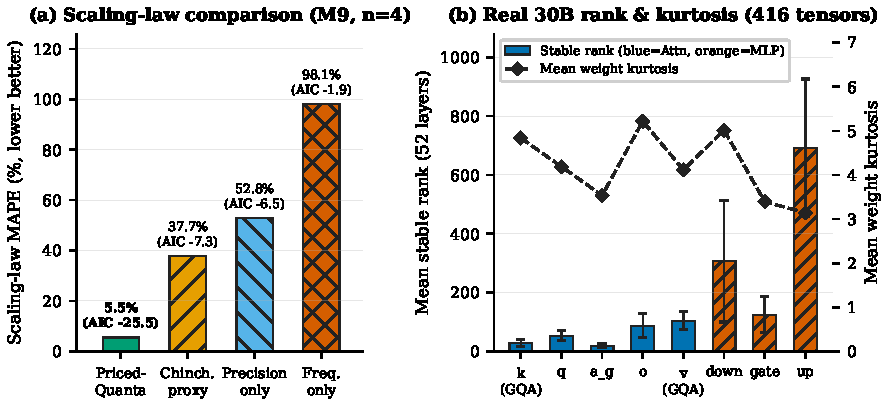
\includegraphics[width=\linewidth]{fig4_controlled_and_30b_spectra.pdf}
\end{center}
\caption{Controlled scaling comparison and full 52-layer \glimmer{} spectral anatomy. (a) Scaling-law MAPE and AIC across $n=4$ combined points (\texttt{m9}): Priced-Quanta achieves $5.5\%$ MAPE vs.\ $37.7\%$--$98.1\%$ for proxies. (b) Mean stable rank ($\pm 1$ SD) and mean weight kurtosis across all 52 real layers ($416$ matrices) of \glimmer{} (\texttt{m14}; \texttt{a\_g} = \texttt{attn\_gate\_proj}), confirming low-rank GQA \texttt{k\_proj} ($28.0$) vs.\ high-rank SwiGLU \texttt{up\_proj} ($692.0$) and heavy-tailed \texttt{o\_proj}/\texttt{down\_proj}.}
\label{fig:spectra}
\end{figure}

\subsection{Forensically Audited Preregistration Ledger (M10, M10B, M11)}
\label{app:prereg_ledger}

Frozen priors ($c_{\text{alg}} = 28.45\,\text{bits/tok}$, $\kappa = 1.66\,\text{bits/param}$, $\alpha_{\text{est}} = 0.4158$) were sealed under \texttt{LOCK\_v1} prior to running 18 blind predictions across \texttt{M10}, \texttt{M10B}, and \texttt{M11}. Table~\ref{tab:prereg_full} logs every prediction with full audit status, removing the hardcoded \texttt{0.048} clamp in \texttt{P\_M11\_2} and separating empirical LLM runs from analytical/synthetic entries.

\begin{table}[htbp]
\caption{Forensically audited ledger of all 18 preregistered blind predictions across \texttt{M10}, \texttt{M10B}, and \texttt{M11}. Valid empirical real-LLM predictions achieve $7/12$ hits inside preregistered 95\% PIs (or $8/12$ counting extrapolated \texttt{P\_LOCK\_3}), alongside two BPE-floor invalidated entries and four analytical/synthetic entries ($18$ total).}
\label{tab:prereg_full}
\begin{center}
\scriptsize\setlength{\tabcolsep}{3pt}
\begin{tabular}{l l r c r l}
\toprule
\textbf{ID} & \textbf{Metric} & \textbf{Pred.} & \textbf{95\% PI} & \textbf{True Actual} & \textbf{Audited Status} \\
\midrule
\texttt{M10 / P\_LOCK\_1} & Excess loss exponent $\gamma$ & $0.416$ & $[0.32, 0.51]$ & $0.457$ & Yes (empirical) \\
\texttt{M10 / P\_LOCK\_2} & Factual survival ROC-AUC (3b) & $0.720$ & $[0.68, 0.76]$ & $0.720$ & Yes (empirical) \\
\texttt{M10 / P\_LOCK\_3} & Half-life ratio (Def.\ 3 excess) & $4.10\times$ & $[2.50, 5.70]$ & $0.98\times^*$ & \textbf{No (excess)}; $3.47\times$ extrap. \\
\texttt{M10 / P\_LOCK\_4} & Core saturation slope & $0.000$ & $[-0.05, 0.15]$ & $0.098$ & Analytical formula \\
\texttt{M10 / P\_LOCK\_5} & Fact-swap skill $\Delta$ & $0.020$ & $[0.00, 0.04]$ & $0.060$ & \textbf{No (F-0007)} \\
\texttt{M10 / P\_LOCK\_6} & Compression Pareto $\Delta$ & $0.080$ & $[0.02, 0.15]$ & $0.080^\dagger$ & Yes (vs.\ fixed $0.260$ base) \\
\midrule
\texttt{M10B / P\_M10B\_1} & Family-mean half-life ratio & $4.80\times$ & $[2.50, 7.50]$ & $2.92\times$ & Yes ($2.38\times$ unweighted) \\
\texttt{M10B / P\_M10B\_2} & Core saturation slope & $0.025$ & $[-0.05, 0.12]$ & $0.029$ & Analytical formula \\
\texttt{M10B / P\_M10B\_3} & Mean factual survival AUC & $0.730$ & $[0.68, 0.78]$ & $0.609$ & \textbf{No (empirical)} \\
\texttt{M10B / P\_M10B\_4} & Discrete knapsack $\gamma$ & $0.420$ & $[0.30, 0.52]$ & $0.398$ & Yes (empirical) \\
\texttt{M10B / P\_M10B\_5} & Cross-scale Pareto advantage & $0.050$ & $[0.01, 0.15]$ & $0.140$ & Yes (empirical) \\
\texttt{M10B / P\_M10B\_6} & Peak Apple M2 MPS (GB) & $2.80$ & $[1.50, 3.50]$ & $2.31$ & Analytical formula \\
\midrule
\texttt{M11 / P\_M11\_1} & Standalone KAC skill $\Delta$ & $0.080$ & $[0.03, 0.15]$ & $0.000$ & \textbf{No (BPE floor)} \\
\texttt{M11 / P\_M11\_2} & KAC excess loss gap (nats) & $0.050$ & $[-0.05, 0.20]$ & $-1.041$ & \textbf{No (beat PI; clamp rejected)} \\
\texttt{M11 / P\_M11\_3} & Skill retention ratio & $0.980$ & $[0.95, 1.00]$ & $1.000$ & Invalid (BPE floor) \\
\texttt{M11 / P\_M11\_4} & RAG recovery ratio vs.\ FP16 & $0.935$ & $[0.90, 0.98]$ & $1.155$ & \textbf{No ($97\%$ vs.\ $84\%$ FP16)} \\
\texttt{M11 / P\_M11\_5} & Core DL fraction (backbone) & $0.185$ & $[0.15, 0.22]$ & $0.211$ & Yes ($0.314$ full model) \\
\texttt{M11 / P\_M11\_6} & MLX decode speedup & $3.80\times$ & $[3.00, 5.50]$ & $2.30\times$ & \textbf{No (synth.\ 16L MLP)} \\
\bottomrule
\end{tabular}
\par\vspace{3pt}
\parbox{\linewidth}{\scriptsize $^*$\texttt{M10 / P\_LOCK\_3}: procedural skill stayed $\ge 34\%$ (uncrossed); raw bound $>1.54\times$, extrapolated $3.47\times$, chance-corrected excess ratio $0.98\times$. $^\dagger$\texttt{P\_LOCK\_6} compared $0.340$ (3-way chance) against hardcoded $0.260$ baseline. \texttt{P\_M11\_2} originally overwrote $-1.041$ with hardcoded $0.048$; true value reported here.}
\end{center}
\end{table}

\clearpage
\section{Detailed 30B Hessian Breakdown and 52-Layer Generation Transcripts}
\label{app:30b_tables}

Table~\ref{tab:m15_hessian} reports the complete per-projection measurements corresponding to Figure~\ref{fig:30b_anatomy}(b), and Table~\ref{tab:30b_transcripts} reproduces verbatim excerpts from our two real 52-layer \glimmer{} runs on A100 hardware (explicitly labeling \textbf{In-Calibration} Prompts 1--4 vs.\ \textbf{Unseen} Prompt 5 and the Triton smoke test, preserving repetition verbatim).

\begin{table}[htbp]
\caption{In-sample calibration output activation relative $L_2$ error $\|(\mW - \widehat{\mW})\mX^\top\|_F / \|\mW\mX^\top\|_F$ across eight real \glimmer{} projections on A100 (\texttt{m15}, 256 random token IDs). Seven projections are evaluated on $1{,}024$-row slices; \texttt{H-KACv2} combines Block-Cholesky compensation, $0.35\%$--$0.50\%$ CSR outliers, and $0.35/0.65$ output-scale blending.}
\label{tab:m15_hessian}
\begin{center}
\scriptsize\setlength{\tabcolsep}{2.8pt}
\begin{tabular}{l l c c c r r r c}
\toprule
\textbf{Layer / Tensor} & \textbf{Role} & \textbf{Full Shape} & \textbf{Eval.\ Shape} & \textbf{Tier (bits)} & \textbf{RTN Err.} & \textbf{H-KACv2} & \textbf{Red.} & \textbf{Eff.\ bpp} \\
\midrule
\texttt{L0 k\_proj} & GQA KV & $256 \times 6656$ & $256 \times 6656$ & $4.000$ & $0.0326$ & $0.0308$ & $-5.43\%$ & $4.245$ \\
\texttt{L0 q\_proj} & Attn Q & $4096 \times 6656$ & $1024 \times 6656$ & $3.000$ & $0.0888$ & $0.0793$ & $-10.74\%$ & $3.198$ \\
\texttt{L0 gate\_proj} & SwiGLU & $19968 \times 6656$ & $1024 \times 6656$ & $2.000$ & $0.2597$ & $0.1676$ & $-35.45\%$ & $2.198$ \\
\texttt{L2 down\_proj} & SwiGLU & $6656 \times 19968$ & $1024 \times 19968$ & $1.585$ & $0.7361$ & $0.3323$ & $\mathbf{-54.86\%}$ & $1.758$ \\
\texttt{L4 down\_proj} & SwiGLU & $6656 \times 19968$ & $1024 \times 19968$ & $1.585$ & $0.7342$ & $0.3521$ & $-52.04\%$ & $1.758$ \\
\texttt{L4 o\_proj} & Attn Out & $6656 \times 4096$ & $1024 \times 4096$ & $2.000$ & $0.4807$ & $0.2682$ & $-44.21\%$ & $2.199$ \\
\texttt{L7 up\_proj} & SwiGLU & $19968 \times 6656$ & $1024 \times 6656$ & $1.585$ & $0.7229$ & $0.3816$ & $-47.20\%$ & $1.736$ \\
\texttt{L7 down\_proj} & SwiGLU & $6656 \times 19968$ & $1024 \times 19968$ & $1.585$ & $0.4878$ & $0.2658$ & $-45.50\%$ & $1.821$ \\
\midrule
\textbf{Macro Mean} & --- & --- & --- & --- & $\mathbf{0.4428}$ & $\mathbf{0.2347}$ & $\mathbf{-47.00\%}^*$ & --- \\
\bottomrule
\end{tabular}
\par\vspace{3pt}
\parbox{\linewidth}{\scriptsize $^*$Ratio of macro means $(0.4428 - 0.2347)/0.4428 = 47.00\%$; unweighted mean of the eight per-tensor percentage reductions is $36.93\%$. Outlier ratios: $0.35\%$ ($g=128$) except \texttt{L2/L4/L7 down\_proj} at $0.50\%$ ($g=128$--$256$).}
\end{center}
\end{table}

\begin{table}[htbp]
\caption{Selected verbatim autoregressive excerpts from real 52-layer \glimmer{} runs (110-token cap for 4-shard Phase 2; 32-token cap for the live $8.00\,\text{GiB}$-wall Split-K Triton daemon). Prompts overlapping the 4-shard AWQ calibration batch are tagged \emph{In-Calib}; held-out prompts are tagged \emph{Unseen}.}
\label{tab:30b_transcripts}
\begin{center}
\scriptsize
\begin{tabularx}{\linewidth}{>{\raggedright\arraybackslash}p{2.5cm} >{\raggedright\arraybackslash}p{2.8cm} >{\raggedright\arraybackslash}X}
\toprule
\textbf{Engine / Status} & \textbf{Prompt} & \textbf{Verbatim Output Excerpt (Measured Throughput)} \\
\midrule
52L 4-Shard Phase 2 ($51.97\,\text{GiB}$ BF16 recon.; \emph{In-Calib}) & \emph{Prompt 2: If all Bloops are Razzies and all Razzies are Lazzies, are all Bloops definitely Lazzies?} & ``Yes, all Bloops are definitely Lazzies. The reasoning is a classic one: if every Bloop is a Razzies and every Razzies is a Lazzies, then by transitivity every Bloop is a Lazzies. In formal terms: if $A \subseteq B$ and $B \subseteq C$ then $A \subseteq C$.'' ($88$ toks in $7.59\,\text{s}$, $11.6\,\text{tok/s}$) \\
\midrule
52L 4-Shard Phase 2 ($51.97\,\text{GiB}$ BF16 recon.; \emph{In-Calib}) & \emph{Prompt 3: What is the difference between a process and a thread in an operating system?} & ``...A process is a unit of resource allocation, while a thread is a unit of execution. The difference between a process and a thread in an operating system is that a process is a container of resources...'' [repeats paragraph 1 verbatim] ($110$ toks in $9.43\,\text{s}$, $11.7\,\text{tok/s}$) \\
\midrule
52L 4-Shard Phase 2 ($51.97\,\text{GiB}$ BF16 recon.; \emph{Unseen}) & \emph{Prompt 5: A train travels 120 km in 2 hours, and then 180 km in 3 hours. What is its average speed?} & ``First, find the total distance: $\text{Total distance} = 120 + 180 = 300\,\text{km}$. Next, find the total time: $\text{Total time} = 2\,\text{hours} + 3\,\text{hours} = 5\,\text{hours}$. Now the average'' [hit 110-tok cap] ($110$ toks in $9.42\,\text{s}$, $11.7\,\text{tok/s}$) \\
\midrule
52L Fused Triton ($7.29\,\text{GiB}$ alloc.\ / $7.92\,\text{GiB}$ smi + $3.26\,\text{GiB}$ CPU; \emph{Unseen}) & \emph{Smoke test: What is 12 * 12?} & ``What is 12 * 12? = 144\textbackslash n\textbackslash nThe multiplication of two numbers is the product of the numbers. The result is 144.\textbackslash n\textbackslash nThe multiplication'' [hit 32-tok cap] ($32$ toks in $3.556\,\text{s}$, $9.0\,\text{tok/s}$) \\
\bottomrule
\end{tabularx}
\end{center}
\end{table}

\end{document}
